\documentclass[a4paper,10pt]{report}
\usepackage{fullpage}
\usepackage{setspace}
\usepackage[margin=1.0in]{geometry}
\usepackage[T1]{fontenc}
\usepackage{mathtools}
\usepackage{url}
\usepackage{booktabs}
\usepackage{graphicx}
\usepackage{fancyhdr}
\usepackage{wrapfig}
\usepackage{caption}
\usepackage[T1]{fontenc}
\usepackage{listings}
 \usepackage{booktabs}
\usepackage[table,xcdraw]{xcolor}


\lstset{language=C++,
  breaklines=true,
  breakatwhitespace=true,
                basicstyle=\small\tt,
                keywordstyle=\color{blue}\ttfamily,
                stringstyle=\color{red}\ttfamily,
                commentstyle=\color{green}\ttfamily,
                morecomment=[l][\color{magenta}]{\#}
}



\begin{document}
\title{3D Procedurally Generated Nature Scene}
\author{Author: Pip Turner - pit@aber.ac.uk  \\
Supervisor: Reyer Zwiggelaar \\
G400 Computer Science \\
CS39440}
\date{\parbox{\linewidth}{\centering%
  \today\endgraf\bigskip
  \textit{Version 1.0}
  }}
\maketitle

\centering
    {\LARGE\bf Acknowledgements}


I am grateful to...

I'd like to thank..

\clearpage
 \raggedright
 
 
%%%
%%% You must sign the declaration of originality. 
%%%
%%% You are submitting this electronically. Therefore, to sign, you 
%%% type your name and date to replace the .... characters. 
%%%
\begin{center}
    {\LARGE\bf Declaration of originality}
\end{center}

I confirm that:

\begin{itemize}
\item{This submission is my own work, except where 
clearly indicated.}

\item{I understand that there are severe penalties for Unacceptable Academic Practice, which can lead to loss of marks or even the withholding of a degree.}
 
\item{I have read the regulations on Unacceptable Academic Practice from the University's Academic Quality and Records Office (AQRO) and the relevant sections of the current Student Handbook of the Department of Computer Science.}
 
\item{In submitting this work I understand and agree to abide by the University's regulations governing these issues.}
\end{itemize}

\vspace{2em}
Name: Pip Turner  \\

\vspace{1em}
Date: 30/04/18 \\

%%% 
%%% We would like to make a selection of final reports available to students that take 
%%% this module in future years. To enable us to do this, we require your consent. You 
%%% are not required that you do this, but if you do give your consent, then we will have 
%%% the option to select yours as one of a number of reports as examples for other 
%%% students. If you would like to give your consent, then please include the following 
%%% text and type your name and date to replace the .... characters. 
%%% 
%%% If you do not wish to give your consent, please remove this from your report. 
%%%
\vspace{1em}
\begin{center}
    {\LARGE\bf Consent to share this work}
\end{center}

By including my name below, I hereby agree to this dissertation being made available to other students and academic staff of the Aberystwyth Computer Science Department.  

\vspace{2em}
Name: Pip Turner  \\

\vspace{1em}
Date: 30/04/18 \\

\setlength{\headheight}{20.2pt}
\pagestyle{fancy}
\setlength{\headsep}{0.2in}
\fancyhf{}

\fancyhead[L]{\leftmark}
\fancyhead[R]{\rightmark}

\fancyfoot[C]{\thepage}

\listoffigures
\listoftables

\tableofcontents
\clearpage



\section{Abstract}
3D Procedural Generation is a way to produce high variety 3D models quickly without manually creating the content. This Project is going to focus on the implementation and subsequent levels of variation of Procedural Generation Algorithms in order to create a cohesive scene. This project will focus on creating nature based content, e.g. Terrain, Trees and Foliage in order to combine them together and create a dense scene which also renders smoothly. 
\clearpage
\chapter{Introduction}
\section{Project Description}

Procedural Content Generation is a broad term referring to the creation of content automatically through algorithmic means~\cite{yannakakis2011experience}. The most popular examples of Procedural Generation are usually the use of it in creating procedurally Generated Worlds, such as No Man's Sky~\cite{nomanssky} - a game which provides the player with a procedurally generated universe to explore. Projects which aim to generate entire planets, or even universes are what initially provided inspiration for this project to be focused around procedural generation - the vast scope, potential and variety of scenes in particular. \medskip


\begin{figure}[h!]
    \centering
  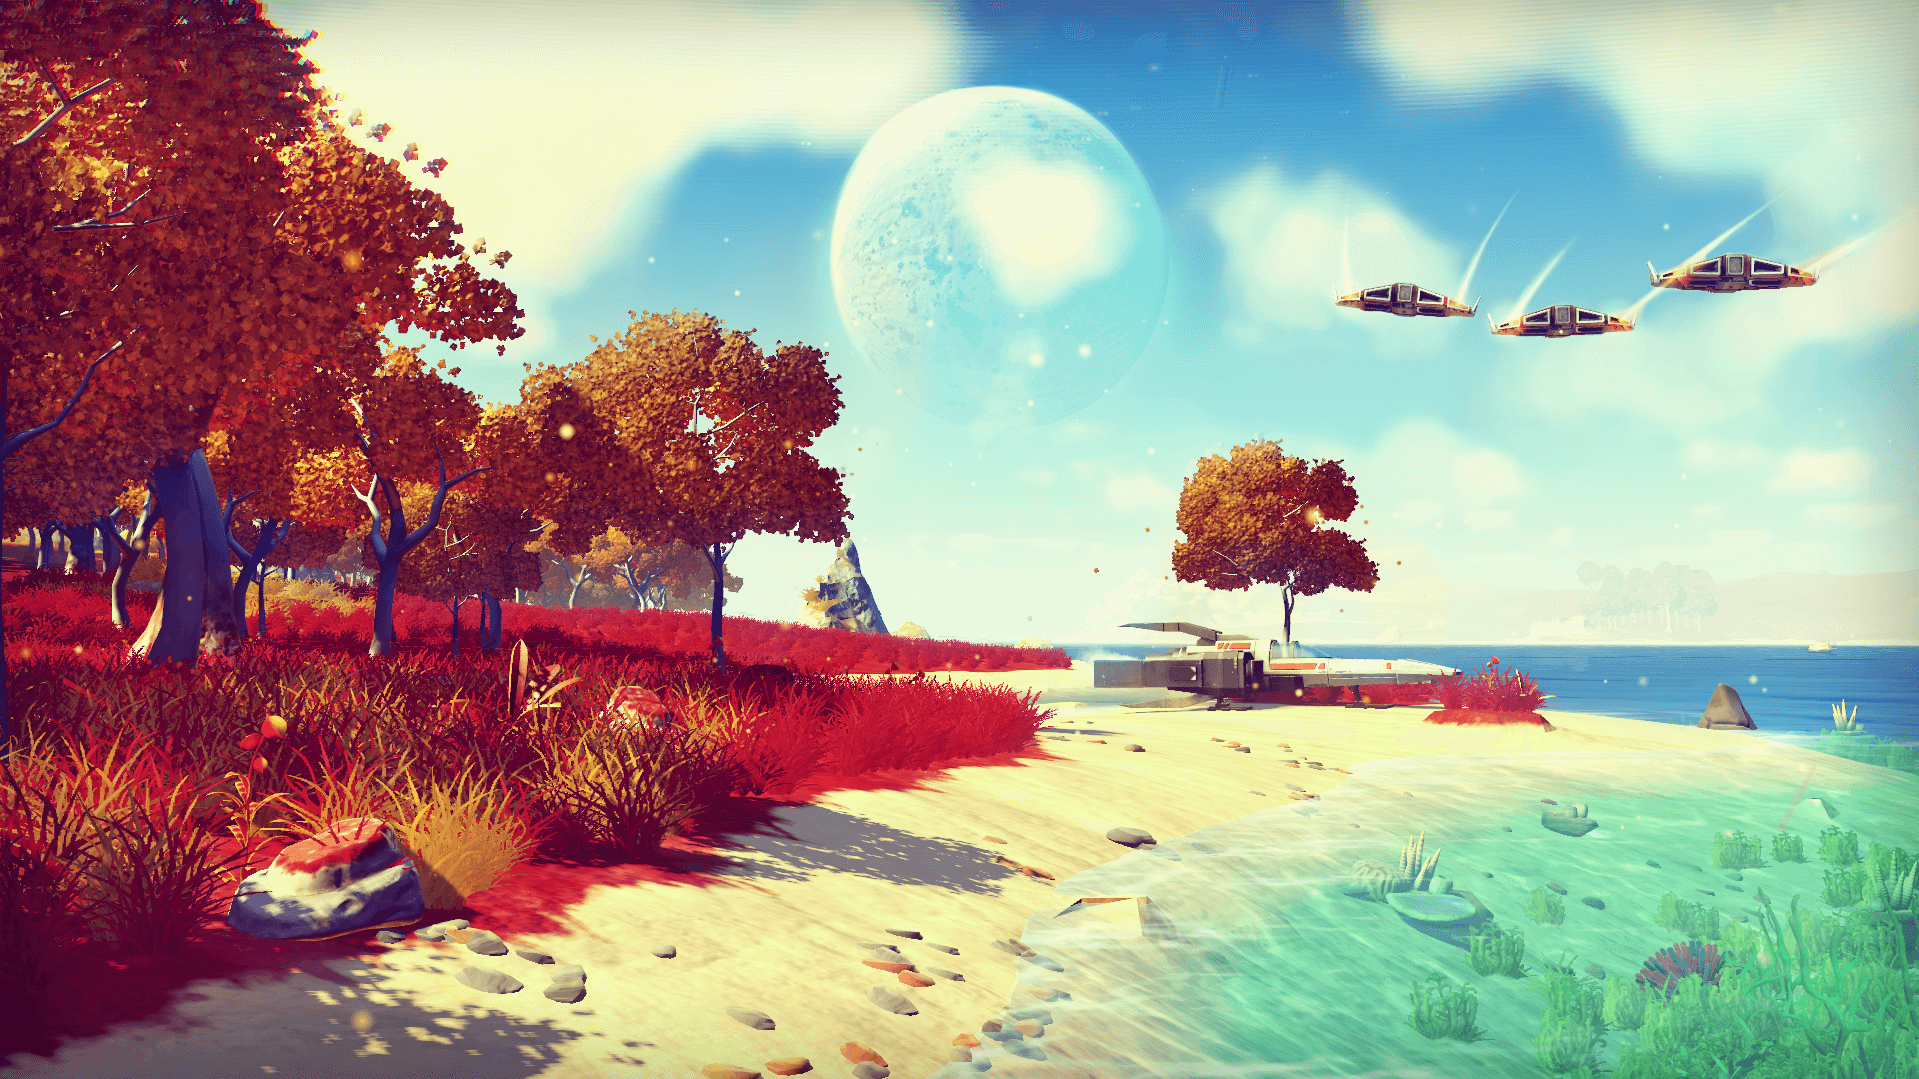
\includegraphics[width=0.9\textwidth]{Images/External/NoMansSky.png}
 \caption{No Man's Sky. Source: https://www.nomanssky.com/press/}
 \label{fig:no_mans_sky}
\end{figure}


This project, therefore is a 3D Procedurally Generated Nature Scene - a small, dense scene utilising procedural content generation techniques to create a  scene which is visibly different each time it is generated. \medskip

However, upon beginning this project, personal knowledge of all areas within this project was limited - this project is as much a personal opportunity to learn low level 3D Graphics and Procedural Generation techniques as it is simply an exercise in implementing them. 

\section{Project Aims}
The aims of the project are as follows:\medskip

\textbf{\textit{Create a 3D Procedurally Generated Nature Scene}} \medskip

The heart of this project is creating a 3D nature scene which is different each time it is generated, using 3D Procedural Content Generation. Rather than creating large, vast swathes of land, this project is instead aiming for a smaller, dense scene in order to generate more interesting landscapes. The smaller the scene, the less content is needed to be generated in order to ensure high levels of variation.\medskip

The main work involved in this aim will be the implementation and subsequent optimisation and use of procedural algorithms. The basic two ingredients needed are Terrain and Trees - this would at the very least show a good understanding and implementation of two to three procedural algorithms. Once these are well implemented, foliage and other details can be added in order to increase the variety of the scene, further progressing the detail and complexity of the scene.  \medskip


\textbf{\textit{Become competent with C++, OpenGL and the core fundamentals of low level graphics}} \medskip

The other main aim of this project is in regards to the skills and technologies learnt whilst working on it. This project was begun with a basic understanding of C++, basic ideas about procedural generation algorithms and no understanding of OpenGL (albeit some basic knowledge of graphics and graphics libraries). Upon completion of this project, there should be a huge jump in knowledge and skills learnt, with a greater appreciation and understanding of C++, procedural generation algorithms and OpenGL.\medskip

\chapter{Research}

In researching into this project, suitable algorithms were needed to be found. Two categories were decided upon - Terrain and Objects on the Terrain. \medskip

\section{Existing Solutions}

\subsection{Terrain}

A major part of this project was selecting and subsequently implementing a terrain algorithm which produced suitably varied and realistic looking terrain. One of the most popular noise generation techniques for Procedural terrain is Perlin Noise~\cite{perlin2002improving} - an algorithm which has been widely used for 3D Graphics, and something which has been instrumental in improving 3D graphics. Whilst it is a popular algorithm, it can be quite computationally expensive and difficult to implement in comparison to other algorithms.\medskip

The supervisor to the project, Reyer Zwiggelaar, suggested looking into Fractal Images, initially suggesting some realistic natural growth based algorithms~\cite{Bilsborough3424}. One of the most widely used Fractal Terrain algorithms is Diamond Square~\cite{olsen2004realtime} - a variation on midpoint displacement. Midpoint Displacement's main issue was that when generating a heightmap it often left "creases" in its landscape, an issue Diamond Square aims to fix by using two stages of midpoint displacement - named Square and Diamond.  \medskip

\begin{figure}[h!]
    \centering
  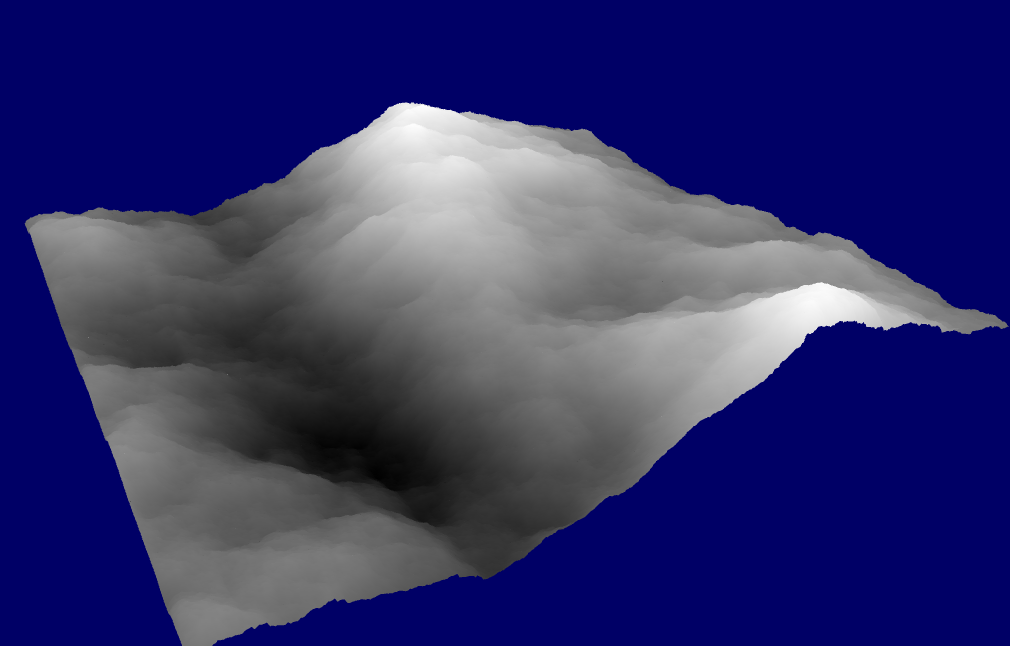
\includegraphics[width=0.5\textwidth]{Images/Screenshots/DiamondSquareGreyScale.png}
 \caption{Diamond Square Terrain with a Greyscale colour applied to it}
 \label{fig:DiamondSquareGrey}
\end{figure}

\subsection{Objects on Terrain}

As well as procedural terrain, in order to ensure a high level of variety, objects upon the terrain are going to also need to be generated. This project will focus mainly on foliage, i.e. Trees, plants and grass. In researching procedurally generated trees two methods were identified as possible implementations - Lindenmayer Systems~\cite{lindenmayer2017} or a Space Colonisation Algorithm~\cite{runions2007modeling}. 

Lindenmayer System is a fractal generation algorithm which builds a fractal by iterating over a string, following a rule set~\cite{prusinkiewicz2012algorithmic}~\cite{crownover1995introduction}. The string can then be interpreted into something drawable. This allows for infinite number of unique fractal patterns to be generated, but most importantly, it can be used to generate trees, bushes and grass like fractals.  

Space Colonisation~\cite{runions2007modeling} works by defining an area in space, filling it with "seeds" (points in space) and "growing" branches towards those points. By doing this, it becomes an incredibly powerful tree generator - generating a huge variety of trees depending on the defined area and the amount of seeds.

\subsection{Optimisation}
This project will require displaying a lot of objects and vertices at once, meaning that optimisation techniques will need to be implemented, as the more vertices on the screen, the lower the frame rate. In order to display the scene professionally, we need to aim for a high frame rate (between 30 and 60).  \medskip

There are a number of big optimisation techniques associated with 3D Graphics. The most applicable optimisation to both Terrain and Trees is Level Of Detail. The further the way an object is from the user, the less detailed the object needs to be. For example, if the player is looking at a far off Mountain, they won't be able to see all of the nooks and crannies on it, only the general shape. This means that we can severely decrease the number of vertices on objects which are far away, whilst keeping high detail on objects which are closer. \medskip

Level of detail is even more relevant when displaying objects like trees, bushes and grass. We can go even further with these using Billboards and Impostors~\cite{jia2013fast}. The basic premise of them is if the tree is far enough from the player for the player to not realise, we can generate an image of the tree and display the image instead. For Example, if we have a tree with five hundred vertices, we can simply display it using six, by mapping the image of the tree onto a quadrilateral polygon made up of two triangles. These images can differ depending on how far away the object is from the player. If the object is very far, we can simply display one image of it, oriented towards the player - this is known as \textit{Billboarding}. However, if the object is a bit closer to the player, we can display an image of the tree at a certain rotation, giving the illusion of perspective to the player. The implementation of Billboards and Impostors can also vary from object to object. Grass, as it is so small can potentially simply be displayed as a Billboard for all of its lifetime. billboard and impostor optimisations can provide huge boost to the frame rate , drastically cutting down the number of polygons in the scene whilst maintaining the illusion of density. \medskip

Objects on the Terrain can also be optimised using instancing and by implementing the Flyweight Design Pattern (\emph{see section 1.5.4}). Instance Rendering allows us to draw the same tree multiple times in different places, whilst only ever storing the data of it once. This saves hugely on memory space.  


\subsection{Design Patterns}

There were no Architectural Design Patterns which seemed relevant for this project. Model View Controller~\cite{vlissides1995design} was considered, but when implementation was theorised, it was found that the pattern simply didn't fit this project - it would be overkill to implement a pattern which lent so heavily on a database on a project which doesn't require any database functionality. \medskip

However, two programming patterns have been identified which are relevant to the project: Flyweight and Command~\cite{nystrom2014game}.\medskip

\emph{\textbf{Flyweight}}\medskip

Flyweight allows you to share common information between objects. This is hugely useful for Trees - they may have the same mesh, colour details or texture. Separating out this data, and then having the instances of the trees carry a pointer to the data can allow for optimised data sharing. \medskip

\emph{\textbf{Command}}\medskip

Command can be used for different inputs the player makes. Instead of hard coding each key press, we can implement command, which abstracts the key press from the command, allowing for easy remapping of keys. This can come in useful for handling movement within the program. 

\section{Suitability of Algorithms}

\subsection{Terrain}

For Terrain, the Diamond Square algorithm will be used. As this project will be completed with limited initial knowledge, choosing an algorithm which is relatively simple to implement, and which produces similar results to Perlin noise is preferable. As Diamond Square is less complex, it also takes less time to generate its height map. However, in comparison to Perlin Noise, it is less flexible - Perlin Noise can be used to generate infinite surroundings on the fly, needing no knowledge of points next to it, whereas Diamond Square Terrain needs to be generated as a whole before it is rendered, meaning that chunks would have to be stitched together to create infinite terrain. However, as the aim of this project is not to provide infinite terrain, but rather a variation on a small part of Terrain, this is not too much of an issue for me. 

\subsubsection{Objects}

When adding objects to the terrain, a high level of variety is preferred. As the time on this project is limited, the Lindenmayer System algorithm will be used, instead of Space Colonisation. In using L-Systems, a high range of different fractals can be used, providing an interesting scene to look at. Lindenmayer Systems are not only fast and have a low memory footprint, they allow for huge variation in not just trees but in creating other objects such as plants, grass and bushes. 

\section{Proposed Implementation}
\subsection{Overview}

In creating this project, it is not only the software implementation which is important to consider, but also the development life-cycle as a whole. A well planned life-cycle can make or break a project. 

\subsection{Software Development}
\subsubsection{Life-cycle}

An Agile Methodology seemed well suited to the project, as the technologies were so new to me, and the project so dynamic in scope. Following a Waterfall style system wouldn't have worked as well, as a rigid plan would not have worked as effectively, due to lesser knowledge of the subject. Agile Methodologies tend to be less rigidly structured, allowing for more flexibility to learn and experiment within the project. \medskip

With this in mind, One Man Scrum Methodology was selected to be used. In a One Man Scrum tutorial, written by Alex Andrews,~\cite{andrews_2017} Andrews discusses the core principles of Scrum - Shipping features regularly, productivity and self reflection \& meaningful iteration. Scrum works by splitting development up into short sections known as "Sprints". Features of a program which need implementing are known as Stories, and each Sprint is focused around completing a specific set of stories, decided upon before the sprint began. \medskip

\begin{figure}[h!]
    \centering
  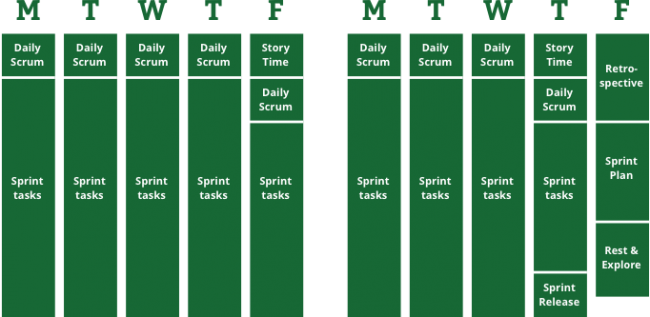
\includegraphics[width=0.9\textwidth]{Images/External/RayWenderlich.png}
 \caption [A proposed two week Sprint plan by Alex Andrews]{A proposed two week Sprint plan by Alex Andrews, sourced from https://www.raywenderlich.com/162654/scrum-one-bring-scrum-one-person-operation . Used with permission.}
 \label{fig:two_week_sprint_plan}
\end{figure}

As seen in Figure~\ref{fig:two_week_sprint_plan}, Andrews proposes a two week Sprint, each day featuring a Daily Scrum, followed by completion of sprint tasks. Each week ends with Story Time, with the final week ending with a Retrospective, Sprint Plan and a time for exploration. The general layout of the two weeks had been organised and put together well, it needed adaptation for this project, due to the small time frame when compared to Andrews. \medskip

\begin{figure}[h!]
    \centering
  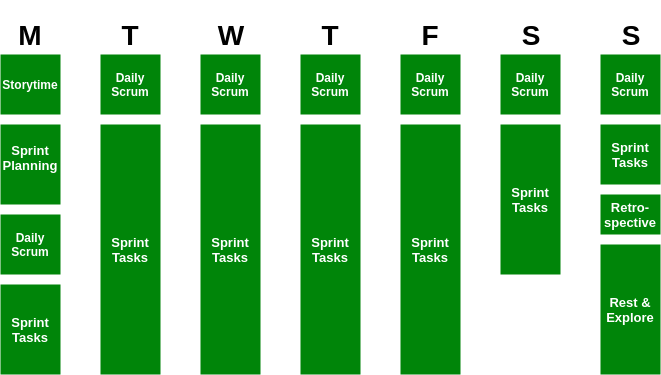
\includegraphics[width=0.9\textwidth]{Images/Charts/Sprint_Plan.png}
 \caption{An adapted version of Alex Andrew's One Man Two-Week Sprint}
 \label{fig:one_week_sprint_plan}
\end{figure}

In Figure~\ref{fig:one_week_sprint_plan}, Andrew's Sprint was adapted into a one week solution, which spanned the entire week rather than five days. \textit{Sprint Release} was removed as the project wouldn't be releasing to the public or testers, so instead commits and features could be built up throughout the sprint. Story planning and Sprint planning were moved to the beginning of the week, to ensure a more focused week throughout. On top of this, the retrospective and exploration were moved to Sunday. \medskip

To support this, a Sprint Log was kept alongside the projects development, which was essentially a record of the daily scrum. Each day a record was kept of the intentions for the day, making sure to relate them to the stories planned and recorded on the Monday. This worked well, as Mondays also tended to be the day a meeting was held with the project's supervisor and Monday tended assigned for Write-Up. Having Monday as a planning and Write Up day gave me a good sense of motivation and a good chance to rest from programming. \medskip

\begin{figure}[h!]
    \centering
  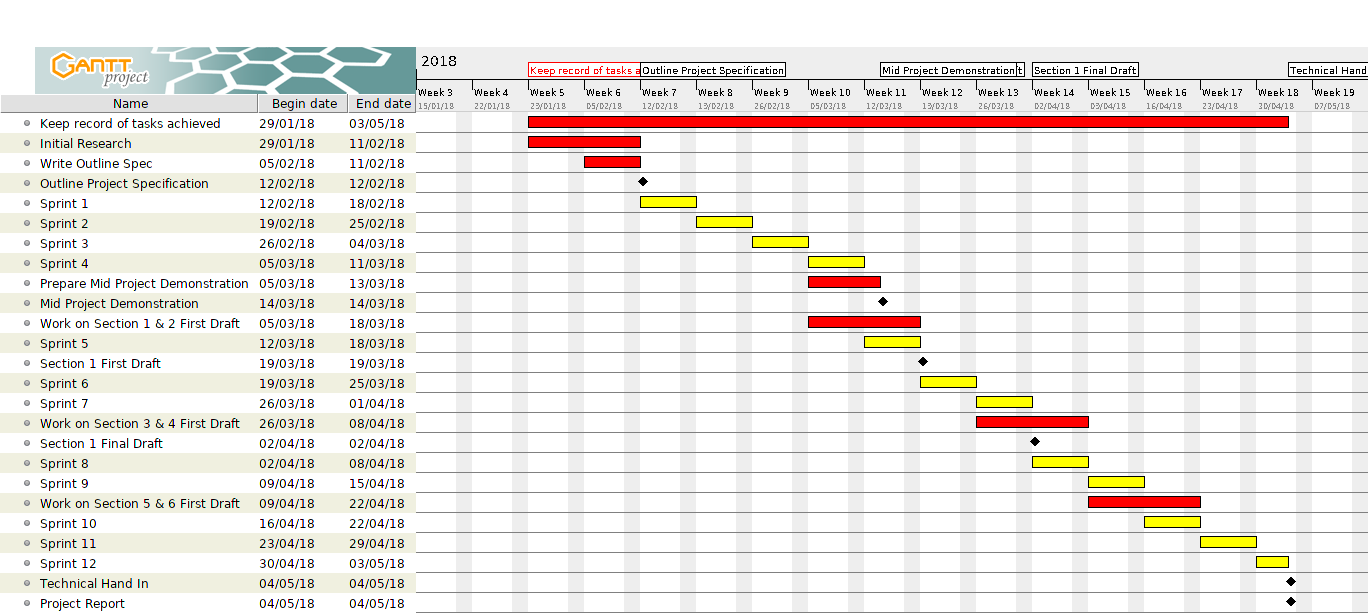
\includegraphics[width=1\textwidth]{Images/Charts/GanttChart.png}
 \caption{A Gantt Chart for the entire project, made with Gantt Project~\cite{gantt}}
 \label{fig:gantt_chart}
\end{figure}


Whilst an Agile Methodology is being used, it does not mean that project planning as a whole can be dismissed. On top of planning at the start of the Sprints, a Gantt Chart (see fig~\ref{fig:gantt_chart} was also used to ensure that the project was on track with both Write Up, Sprints and Project deadlines. This, coupled with the Project Outline Spec, provided a lot of insight into how to shape the project was shaped, and ensured that it would be finished on time. \medskip


\section{Relevant Technology}

\subsection{C++}

This project will be coded primarily in C++, as an aim of the project is to become more familiar and more comfortable with C++. As well as this, C++ has its own benefits - it tends to be very fast, is very often used for graphics coding due to the powerful libraries available, such as DirectX~\cite{directx_website}, OpenGL~\cite{OpenGL_website} and Vulkan. When writing in C++, it was decided to follow Google's Style Guide's~\cite{google_c_style_guide} naming conventions, in order to ensure a coherent and consistent code base.

\subsection{OpenGL}
In choosing C++, there were multiple Graphics APIs to choose from. DirectX's Direct3D was disregarded due to its limited application in terms of cross platform - it only being compatible with Windows based hardware. Vulkan, intended to be a "Next Generation OpenGL" was also eventually disregarded as an option. Despite being newer, and potentially more powerful than OpenGL, it is also more verbose and lower level and therefore harder to pick up. As the project is being made with relatively little experience with 3D Graphics APIs, previously only having experience with  high level JavaScript libraries beforehand, it was more advisable for to use OpenGL - a cross platform graphics API. Using OpenGL gives me a better way to learn the fundamentals of low level graphics, as well as the option to move onto Vulkan in the future.

\subsection{GLSL}

GLSL, or \textit{OpenGL Shading Language} is the language used by OpenGL for its shaders. Whilst shaders wont be focused on too much during the project, they are still needed by necessity, and so some GLSL will be used.

\subsection{CLion}
CLion~\cite{clion_jetbrains} was selected as the IDE of choice, as it offers powerful tools for a programmer, as well as a very slick user interface. Having had previous positive experiences with Jetbrains products, using CLion for this project seemed like an obvious choice.

\subsection{LaTeX}
In order to write this report, LaTeX~\cite{latex_website} was used, due to its professional rendering of documents. Overleaf.com~\cite{overleaf_website}, a cloud based LaTeX editor was used to edit the report in, which ensured that the report's data couldn't get lost, as it also had Github integration.

\subsection{Draw.io}
Any charts used in this document were generated using draw.io~\cite{draw_io}, an easy to use chart maker, which provided the option to save to cloud based providers, again allowing for an easy way to keep the chart data safe. 

\subsection{Version Control - Git \& Github}
This project was made using Git as version control, being saved to a private repository on Github~\cite{github}. This allowed easy rollbacks where needed, as well as ensuring that the project's data would not be lost, as it is saved on the cloud. In addition to this, Overleaf was used for version control and cloud saving for the report - it also uses a Git backend for this.

%%%%%%%%%%%%%%%% NEW CHAPTER %%%%%%%%%%%%%%%%

\chapter{Design and Implementation}

\section{Overall Architecture}

The project will perform the following processes in order when run: \bigskip

\textbf{Open a Window} \par
Firstly, the project will open a window, using GLFW~\cite{berglund2006glfw}, in order to show that it is running. \medskip

\textbf{Generate Diamond Square Heightmap} \par
The project will then generate a Diamond Square Heightmap, as the heights generated will inform a lot of the rest of the project. \medskip

\textbf{Generate Terrain Vertices} \par
The project will then convert the Heightmap into triangle based vertices, passing it to OpenGL's vertex buffer. \medskip

\textbf{Generate Terrain Colours} \par
The project will then generate the terrain colours, based off of the terrain's height. \medskip

\textbf{Generate L-Systems} \par
The project will then generate L-System fractals \medskip

\textbf{Generate L-System Positions} \par 
The project will then generate the positions of the fractals \medskip

\textbf{Draw Loop} \par
The project then enters the draw loop, not leaving until "Esc" is pressed. \medskip

\textbf{Check for Key Input} \par 
The project then checks for any input from the user, responding accordingly. \medskip

\textbf{Compute Camera MVC} \par 
The project then computes the camera's view matrix based on mouse and keyboard input. \medskip

\textbf{Draw Vertices} \par 
The project then draws the terrain, followed by trees. \medskip

\section{Software Structure}
As this project is so reliant on C++ and OpenGL, these two technologies dictate the Software's structure. C++ is primarily an Object Oriented Language, with OpenGL being a state machine and Graphics API, a structure already built into it. \\

\begin{figure}[h!]
    \centering
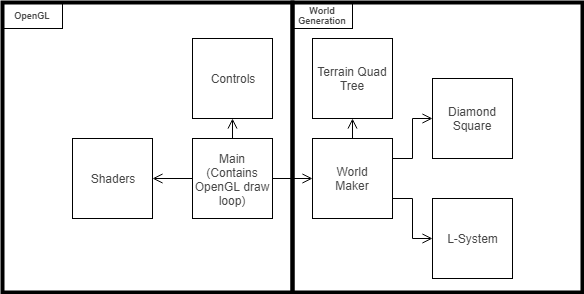
\includegraphics[width=0.8\textwidth]{Images/Charts/Architecture.png} 
\caption{Diagram illustrating the architecture of the project}
\label{architecture}
\end{figure} 

In order to keep the project organised, the code was split up into two distinct parts - specific OpenGL related code, and procedural generation. As seen in fig~\ref{architecture}, OpenGL draw loop (\textit{main.cpp in the source code) controls the project} controls the OpenGL related code, whilst World Maker controls the Procedural Generation aspects of it. Separating out these two parts helped motivate a code base which was both modular in design (allowing for easily changeable code), and created an architecture which allowed for easy feature additions. \\

Diamond Square and L-Systems were split off into their own object classes, in order to allow for easy creation and generation of them, as well as to enable a more modular code design. A modular design philosophy has driven the majority of code in this project. In designing each class, functionality was separated into different, independent methods, allowing for a good deal of re-usability and flex-ability in bug fixing. C++'s vectors played a big part in ensuring the flexibility of code. Instead of relying on fixed length arrays, which create quite static code, using vectors (which can be accessed in a similar way to arrays if needed) allowed for a more dynamic and easily added to program. \\

\begin{figure}[h!]
\centering
  \fbox{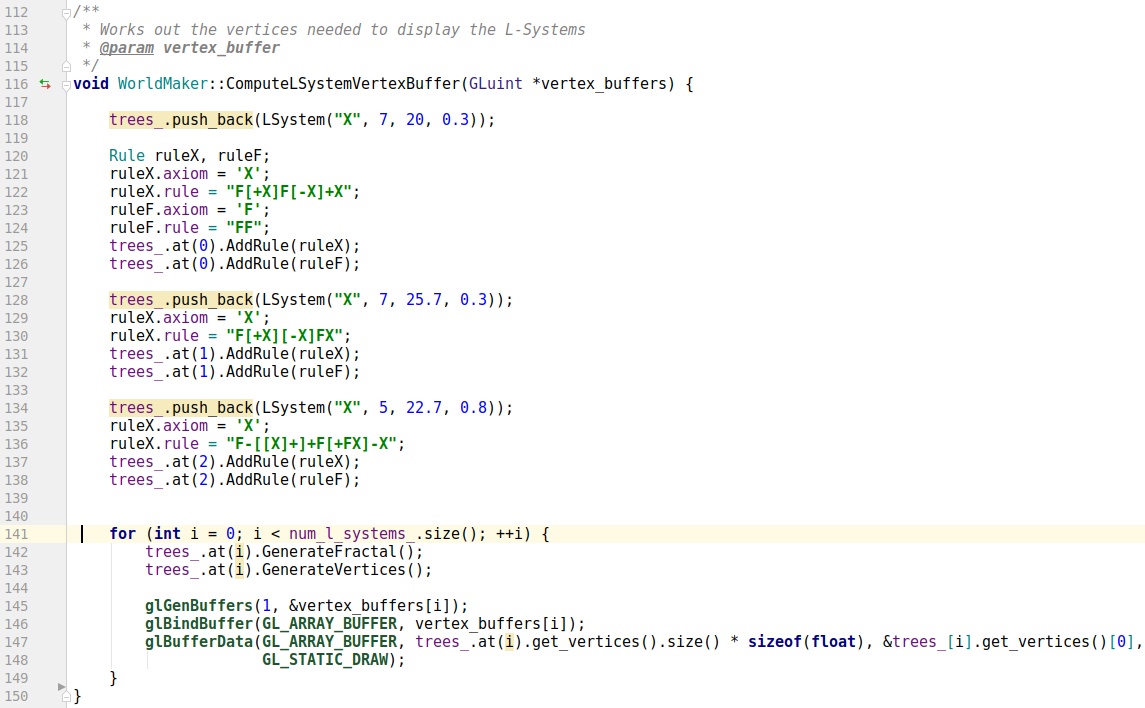
\includegraphics[width=1\textwidth]{Images/Code-Snippets/LSystemGeneration.png}}
 \caption{The method which defines and generates L Systems, an example of the usefulness of modularity.}
 \label{fig:tree_generation}
\end{figure}

As seen in fig~\ref{fig:tree_generation}, modularity can be extremely useful. This method has three L-Systems defined, but we can theoretically define as many L-Systems as the vector (a class-private single dimension vector instance variable named \textit{trees\_} ) can hold. Once all L-Systems are defined, the program then iterates over the vector storing them, generating then and then binding the vertices to OpenGL's vertex buffer. The program will simply display as many L-Systems as defined, without the need for any additional code. In separating out functionality into modular classes and functions, it is not an issue to tweak and adjust the program once the overall structure has been implemented.

\subsection{Initial Class Structure}
The classes were initially designed as follows. Quadtrees had not yet been considered upon initial class design. As this was an initial design, this was intended more of a rough outline rather than a concrete architecture. The idea was that the project could build from the core intention of this design, rather than rigidly sticking to it. 

\subsection{Main.cpp}

The class Main.cpp will initially be based off of the tutorials found on http://opengl-tutorial.org~\cite{opengl_tutorial}.

\subsubsection{Instance Variables}
\textit{GLFWwindow window.} 

This class will only store a variable of the window being used, as it is needed for OpenGL's draw loop.
\subsubsection{Functions}
\textit{int main()}\\
This class will contain the "main" function for the project, the designated start of the program. \\

\textit{void OpenGLMagic}\\
This method will set up what is necessary for OpenGL to draw the world, before entering the draw loop.


\subsection{DiamondSquare.cpp}

This class will handle all things to do with Diamond Square generation. 

\subsubsection{Instance Variables}

Diamond Square will store the heightmap initially generated, allowing for it to be easily accessible to other classes.

\subsubsection{Methods}

\textit{GenerateHeightMap}\\
This method will generate the heightmap, by following the Diamond Square algorithm. \medskip

\textit{Generate Vertices}
This method will take the heightmap generated, and from it generate vertices which can be interpreted by OpenGL to draw triangles. 

\subsection{L\_System.cpp}
This class handles all things to do with L\_System generation.

\subsubsection{Structs}

\textbf{Rule}\\
\textit{char axiom}\\
\textit{string rule}\medskip

The rule Structure helps us represent rules to apply to the L-System string. For example, in the rule "B -> AB", "B" is the axiom, and "AB" is the rule.

\subsubsection{Instance Variables}
\textit{string seed} - the initial seed the L\_System grows from\\
\textit{string fractal string} - the final string after iterations\\
\textit{int no\_of\_iterations} - the number of times the string will be iterated over\\
\textit{angle\_mod} - the angle of which to turn\\
\textit{rules} - all the rules to be applied to the seed\\
\textit{vertices} - the eventual interpretation of the final string as a set of vertices\\

\subsubsection{Methods}

\textit{Generate Fractal}\\

This method will take the seed, iterate over it  "no\_of\_iterations" times, following the rules stored in the class.

\textit{Generate Vertices}\\

This method will take the final fractal string and interpret it according to the rules of Turtle Graphics.

\clearpage

\section{Final Design}

Much like in fig~\ref{architecture}, the final design is split up into two parts - the classes relevant to OpenGL, and the classes generating the vertices to push to OpenGL. Due to the size of the full UML chart, these two sections have also been broken down into separate charts.

\begin{figure}[h!]
\centering
  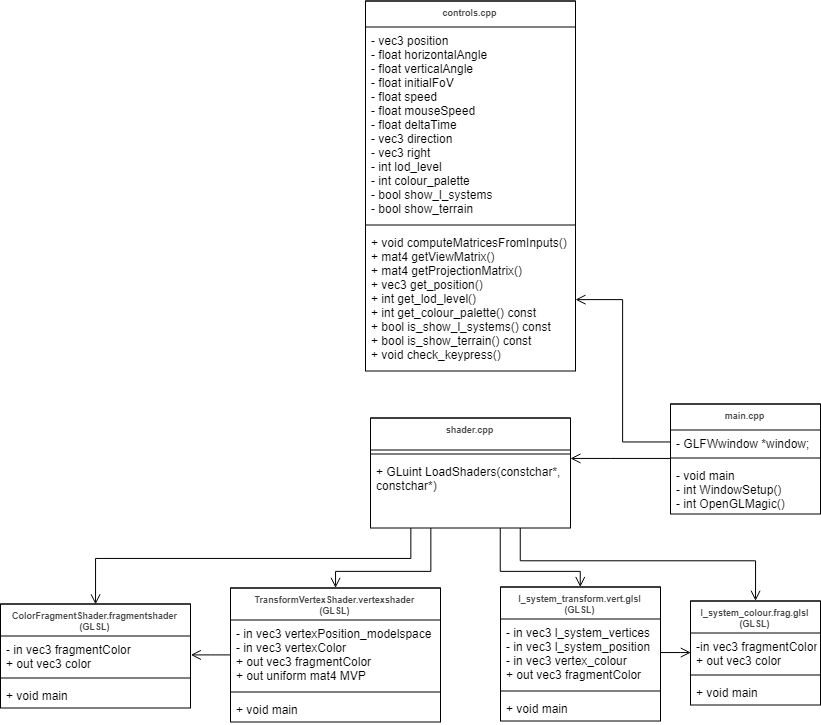
\includegraphics[width=1\textwidth]{Images/Charts/OpenGL_UML.png}
 \caption{UML of classes relating to OpenGL}
 \label{fig:opengl_uml}
\end{figure}


\subsection{OpenGL Related Class Structure}

The following classes are related to the OpenGL half of my project. They include the main class (\textit{main.cpp)}, Shaders(\textit{shader.cpp}, \textit{ColorFragmentShader.fragmentshader}, \textit{TransformVertexShader.vertexshader}, \textit{l\_system\_colour.frag.glsl}, \textit{l\_system\_transform.vert.glsl}, and the class which recalculates the camera's MVP, as well as handles user input (\textit{controls.cpp}). 

\subsection{main.cpp} 

This class controls everything else in the program, as well as sets up a window and then displays the vertices needed into the window. Whilst this could have been abstracted out into a different class which this class calls, it would have been functionally identical, so the decision was made to keep the code in \textit{main.cpp}. In the method \textit{OpenGLMagic()}, it uses the method in shader.cpp, passing into it all four GLSL shaders. \\

This class sets up a window, before setting up everything needed to display the vertices in the window, using the World Maker class. Then each draw loop, it checks for user input, computes the camera's position, before drawing the terrain followed by the L-Systems.


\subsection{controls.cpp}

This class recalculates the camera's MVP (Model, View, Perspective) matrix and handles user input. Whilst this class was intially a class brought over from work done on tutorials, it was eventually reworked into an object, in order to make code easier to read. As well as this, it keeps track of user input, to allow for functionality such as changing the Level Of Detail displayed on screen, or changing the colour palette. 

\subsection{shader.cpp}
This class was provided by the tutorials followed. It compiles the shaders, passing them to the driver, before returning a shader ID for us to access them by. 

\subsection{TransformVertexShader.vertexshader}
This shader was provided by the tutorials followed. It takes in a vertex position and colour, outputs the position multiplied by the MVP matrix, and passes out the color to the fragment shader.


\subsection{ColorFragmentShader.fragmentshader} This shader simply takes in the color and then outputs it again. It is here more for future proofing, so we can easily have more complex shaders in the future.  

\subsection{l\_system\_transform.vert.glsl}
Unlike TransformVertexShader, this shader takes in the l\_system vertices, and then a separate vector containing its position. It then positions the mesh in the vector containing its position.


\subsection{l\_system\_colour.frag.glsl}
This shader is identical to ColorFragmentShader.fragmentshader. It only exists again for future proofing the project. 


\clearpage
\subsection{Procedural Generation Class Structure}

\begin{figure}[h!]
\centering
  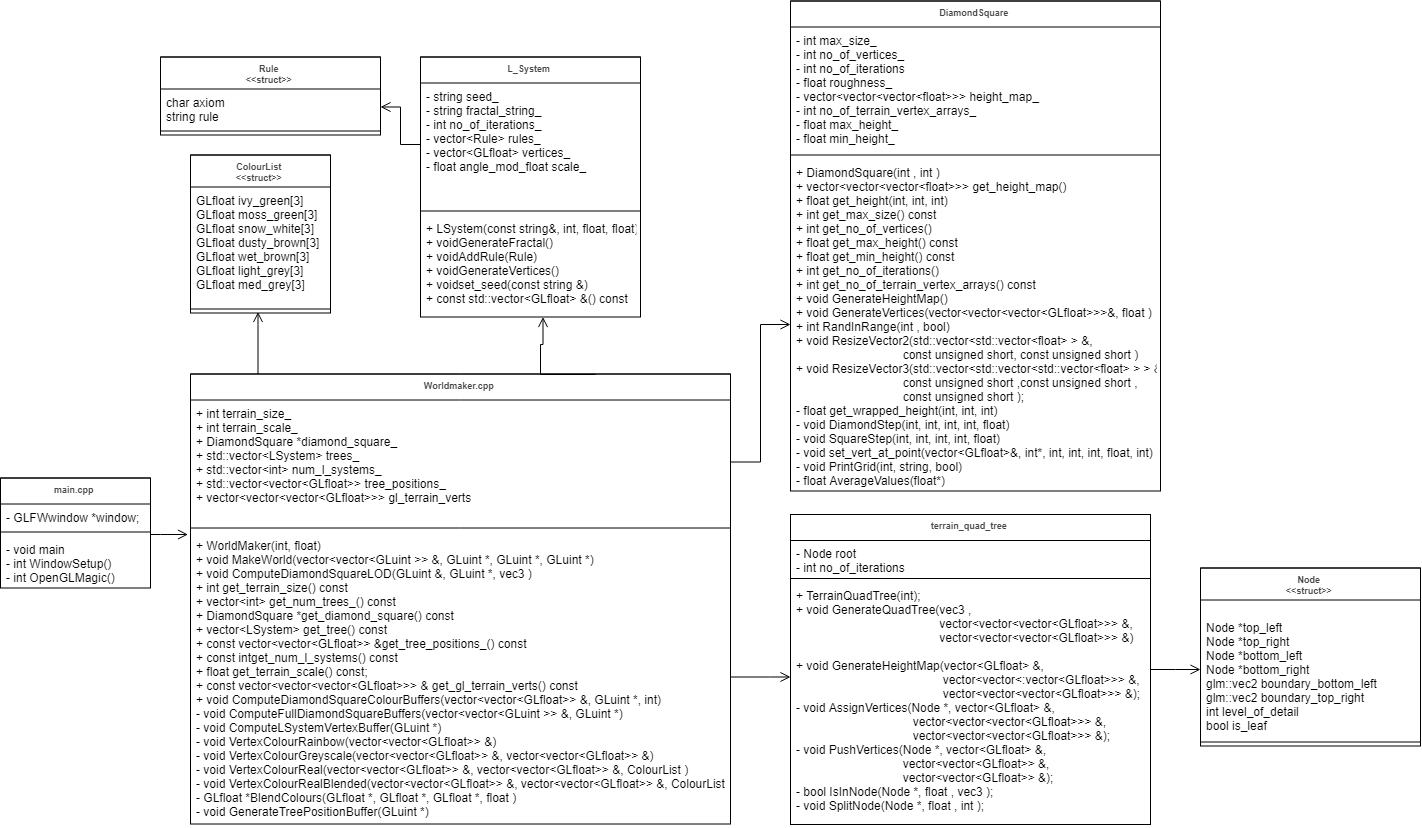
\includegraphics[width=1\textwidth]{Images/Charts/GenerationUML.png}
 \caption{UML of classes relating to OpenGL}
 \label{fig:GenerationUML}
\end{figure}

The following are related to the Procedural Generation part of the project.

\subsection{world\_maker.cpp}
WorldMaker is integral to the entire project. It controls the generation of everything within the world, specifying the order in \textit{MakeWorld()}, which takes in pointers to GLuints storing the ids for each vertexbuffer. \textit{MakeWorld()} first calls \textit{ComputeFullDiamondSquareBuffers()}, which gets DiamondSquare to generate the terrain vertices, before binding them to the vertex buffer. It then calls \textit{ComputeDiamondSquareColourBuffers()}, telling it to initially generate the colours in the blended colour palette. Once the colours have been generated, \textit{MakeWorld} then calls \textit{ComputeLSystemVertexBuffer()}, which generates the L-System vertices needed, followed by the generation of positions for the trees.

\subsection{struct ColourList}
This struct simply provides a point of access to the list of colours used to colour in the landscape.

\subsection{diamond\_square.cpp}

This class holds all the methods needed for generating a Diamond Square based Height Map, and converting that heightmap into vertices. When the constructor is called, once it has intialised all variables it then calls \textit{GenerateHeightMap()}, which generates \textit{n} number of height maps (where \textit{n = no\_of\_iterations}). Each iteration is representative of a different Level of Detail. \textit{GenerateVertices()} is called during world generation. It iterates over every heightmap generated, producing its equivalent vertices to display. 

\subsection{l\_system.cpp}
l\_system.cpp holds all the methods needed to generate one Lindenmayer System fractal. An L-System is first built up by defining the seed, number of iterations, angle modifier and scale in the constructor. Rules are then added, before generating the final iteration of the fractal string, with \textit{GenerateFractal()}. After generating the fractal, \textit{GenerateVertices()} is called, which generates the vertices to represent the tree through OpenGL.

\subsection{struct Rule}
This struct holds an axiom and a rule of which the axiom is replaced by. 

\subsection{terrain\_quad\_tree.cpp}
terrain\_quad\_tree.cpp is an implementation of a Quadtree. It simply has two instance variables, the Quadtree's root, and the number of iterations the Quadtree will run for. This class is a proof of concept for Level Of Detail tessellation. Whilst in practice the class itself is not optimised enough for live implementation, if it were to be used, GenerateQuadTree() is first called, which iterates over the heightmap, generating a quad tree, with smaller nodes being closer to the camera's position. Once it has been generated, GenerateVertices() is then called, which generates a set of vertices of stitched together heightmaps, as a quadtree. 

\subsection{struct Node}
Node is a struct used in terrain\_quad\_tree.cpp, which holds four nodes (representative of the Node's potential four children), details of its boundary, what level of detail it is and whether it is a leaf or a parent.


\clearpage

\section{Algorithms}
\subsection{Diamond Square}
The Diamond Square algorithm~\cite{miller1986definition}, is an algorithm which randomly generates fractal based terrain, iterating over terrain using two steps - Diamond and Square. \medskip 

\begin{figure}[h!]
    \centering
  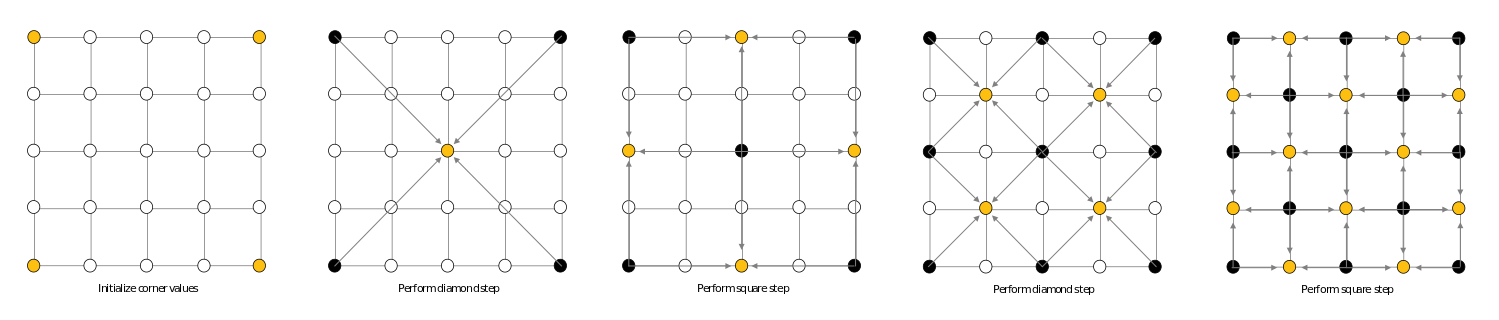
\includegraphics[width=0.9\textwidth]{Images/External/Diamond_Square.png}
 \caption[Diamond Square steps, by Christopher Ewin]{Diamond Square steps, by Christopher Ewin CC BY-SA 4.0, https://commons.wikimedia.org/w/index.php?curid=42510593}
 \label{fig:diamond_square_steps}
\end{figure} 

Diamond Square is performed on an initially flat grid. The steps (as pictured in fig~\ref{fig:diamond_square_steps}) are as follows:

\begin{enumerate}
\item \textit{Initialise corner values}
\item \textit{Diamond Step}
\item \textit{Square Step}
\item \textit{Reduce step size} 
\item \textit{Repeat Steps 2-4 while step size is greater than 1}
\end{enumerate} 

The Step Size (used in both the Square Step and the Diamond Step) is initialised to the grid's width -1. The Diamond step takes each square in the grid, of width Step Size, and sets the midpoint of the square to the average of its corner values, in addition to a random value (which decreases alongside Step Size). The Square step takes each diamond in the gird of width Step Size and sets the midpoint of the diamond to the average of its corner values, in addition to a random value (which decreases alongside Step Size). \medskip

One of the main issues with Diamond Square are edge values - whilst all other values gain their height from the average of 4 other values, edge cases don't have enough data around them for this. There are two solutions to this - use the 3 available values, or wrap round the values to the other side of the grid. 

\subsection{Lindenmayer Systems}


\begin{wrapfigure}{r}{4cm}
\centering
  \fbox{
\includegraphics[width=0.11\textwidth]{Images/Charts/AB_Example.png}}
 \caption{Diagram illustrating an L-System's iterative process}
 \label{fig:l_system_AB}
\end{wrapfigure}


Lindenmayer System is a String manipulation algorithm, which recursively iterates over a String according to a set of rules in order to generate a String representation of a fractal pattern. It's steps are as follows:


1. Define initial String seed
2. Define the L-System's rules
3. Iterate over the string \textit{n} times, following the defined rules


A simple example:\medskip

\textbf{Seed:} \textit{"A"}

\textbf{Rule 1:} \textit{A $\rightarrow$ AB}

\textbf{Rule 2:} \textit{B $\rightarrow$ A}


Iteration 0: A

Iteration 1: AB

Iteration 2: ABA

Iteration 3: ABAAB

Iteration 4: ABAABABA

Iteration 5: ABAABABAABAAB\medskip



In Figure \ref{fig:l_system_AB}, Patterns can be generated easily and quickly. The next stage of Lindenmayer Systems is interpreting these patterns into something we can draw - this is achieved using "Turtle Graphics". The book, The Algorithmic Beauty of Plants~\cite{prusinkiewicz2012algorithmic} contains a comprehensive explanation of Lindenmayer Systems including these rules for 3D Lindenmayer Patterns:\medskip

F: Move forward, by step \textit{d} and orientation \textit{n}. A line between {x, y, z} and {x', y', z'} is drawn. \\

f: Move forward, by step \textit{d} and orientation \textit{n}. \\

+: Turn left by angle $\sigma$ along the xy axis (using the z rotation matrix)\\

-: Turn right by angle $\sigma$ along the xy axis (using the z rotation matrix)\\

\&: Pitch down by angle $\sigma$ along the xz axis (using the y rotation matrix)\\

$\wedge$: Pitch up by angle $\sigma$ along the xz axis (using the y rotation matrix)\\

\textbackslash: Roll left by angle $\sigma$ along the yz axis (using the x rotation matrix)\\

/: Roll right by angle $\sigma$ along the yz axis (using the x rotation matrix)\\

|: Turn around along the xy axis (180 degrees using the z rotation matrix)\\

[: Push the current state of the turtle onto a stack\\

]: Pop a state from the stack and apply it to the turtle\medskip

These rules expand the usefulness of Lindenmayer Systems and are especially useful for this project, as they allow for branching structures, allowing us to create trees.

\clearpage
\subsection{Terrain Level Of Detail}

\begin{figure}[h!]
    \centering
  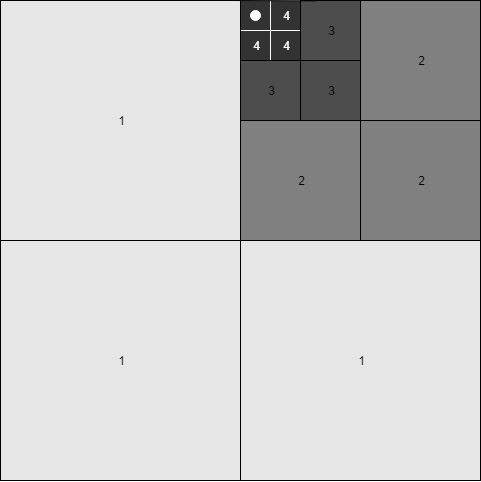
\includegraphics[width=0.3\textwidth]{Images/Charts/QuadTree.png}
 \caption{Quadtree example. The darker the shade, the higher detailed the terrain in that area. White circle denotes where the camera is.}
 \label{fig:quad_tree}
\end{figure}

One of the biggest optimisation's to be made for this project will be Terrain Level Of Detail (Level Of Detail). This optimisation is split into two parts - the generation of the different levels of detail, alongside the combining of them, and deciding the amount of vertices to display. This could be done dynamically, but lacking the time and definition  to implement the complexity of a dynamic terrain renderer, instead we have something easier to use. Diamond Square, upon generating its terrain automatically generates different levels of detail which can easily used for this algorithm. These levels of detail can then be stitched together, depending on the technique used for Level Of Detail display. \medskip

An often used technique for deciding what Level Of Detail each chunk of terrain will be is using a Quadtree system to split up terrain~\cite{pajarola1998large}. A Quadtree is a tree structure where each node has exactly four children. As seen in Figure~\ref{fig:quad_tree}, this tree structure can easily be applied to splitting up terrain. In Figure~\ref{fig:quad_tree}, each shade (as denoted by the numbers) represents a different Level Of Detail - the darker the shade, the higher the detail. whilst this can easily work, the main problem are cracks between each chunk of terrain. This can potentially be solved by working averaging the edges to the midpoint of each other, but this could potentially prove problematic as each edge has different numbers of triangles. A crude solution would involve moving the edge vertices of the edge triangles up to the same elevation as the edge of their neighbouring chunk. \medskip

A solution to this problem is known as Restricted Quadtree Triangulation~\cite{pajarola1998large}. This works by restricting triangulation to points that match. Whilst this is definitely a more elegant method, time restrictions have stopped me from implementing this. 

\subsection{L-System Rendering Optimisation Techniques}
L-Systems when displayed on screen may use a lot of vertices, especially if displayed using 3D Primitives such as cylinders. In order to reduce the amount of vertices displayed we can use a similar technique to Terrain Level Of Detail; the further away the trees are from the camera, the less detail they display. However, unlike the terrain, we cannot simply reduce the number of vertices in the tree. Instead, we use Billboards and Impostors. When the tree is far enough away, we simply replace it with a two dimensional sprite of the orientation of the tree facing you - known as an \textit{Impostor}. A billboard is used, when the tree is further away. Rather than choosing from a number of orientations of the tree to display, there is simply one, which is rotated to constantly face the camera. Due to the distance of the tree from the camera, the angle of which it is viewed does not matter, so we can simply display one orientation of it to the user.


\chapter{Sprints}

At the start of each week, stories/sprint goals were set out of what was the week was aiming to achieve. The structure of a story was roughly:\medskip

\textit{"As a \_\_\_\_\_\_, I need to \_\_\_\_\_\_, so that I can \_\_\_\_\_\_"}

\section{Sprint 1 (12/02/18 - 18/02/18)}

\subsection{Sprint Goals}

\begin{enumerate}
  \item \textit{As the Developer, I need to become more familiar with C++ and OpenGL, so that I can properly get going with the project. I will achieve this through research into the implementation of OpenGL and going through an OpenGL tutorial which I have already begun.}
  
  \item \textit{As the Student, I need to start thinking about my Major Project's Report, so that I will not have an overload of writing at Easter. I will achieve this by setting out the sections of my report and making a start on the introduction.}
  \item \textit{As the Developer, I need to have a strong idea of how I am going to implement my project, in order to prevent floundering and confusion later on. I will achieve this through more Software Engineering Design Pattern and Architectural Pattern research. }
\item \textit{As the Developer, I need a good idea of how much time I have left before my various deadlines, so that I can increase my drive to work. I will achieve this through further improving my Gantt Chart, namely adding more strong Major Project deadlines. }

\end{enumerate}

\subsection{Sprint Summary}

The first sprint's main aim was to lat a good foundation on which to build the rest of my project. This was achieved through working through a set of OpenGL Tutorials~\cite{opengl_tutorial}, tweaking the project's Gantt Chart and Outline Spec, researching into potential Design Patterns (Model View Controller), learning more about OpenGL's general architecture, and more 3D Graphics basics (in particular, Model, View and Projection). \medskip

A significant accomplishment was being able to display two different items in OpenGL. Whilst this may seem trivial, and an easy accomplishment, it meant the culmination of the knowledge learnt throughout the entire week - representing objects through vertices, Vertex Buffers and Colour Buffers, basic C++ syntax, and OpenGL syntax.\medskip

\clearpage
\section{Sprint 2 (19/02/18 - 25/02/18)}

\begin{figure}[h!]
    \centering
  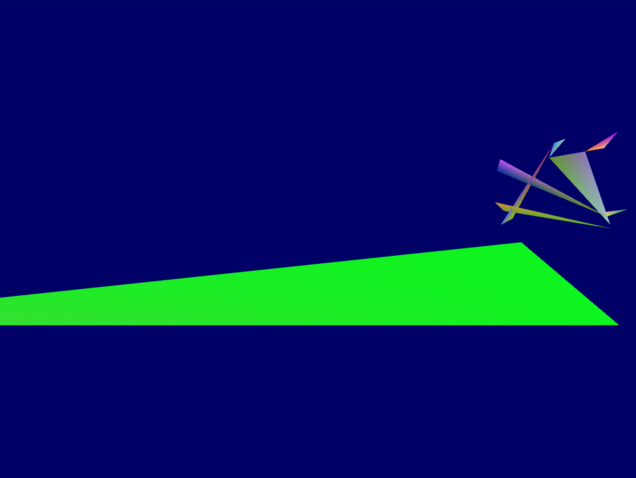
\includegraphics[width=0.5\textwidth]{Images/Sprint-Images/Sprint2-1.png}
 \caption{Initial triangles displayed. OpenGL essentially displaying garbage as both major algorithms within the DiamondSquare class were incorrectly implemented}
 \label{fig:sprint2-1}
\end{figure}

\subsection{Sprint Goals}
\begin{enumerate}
    \item \textit{As the Developer, I need to set up a private git repository so that I can properly use version control in order to avoid major project screwups.
    }
    \item \textit{As the Developer, I need to begin implementation, in order to hit deadlines and be prepared enough for my mid project demonstration.}
    \item\textit{As the Student, I need to continue working on my Report and identify which sections to work on this week so that I don't leave it to the last minute.}
    
\end{enumerate}

\subsection{Sprint Summary}

The second sprint's main aim was to finish building the foundation which was begun in the first sprint, whilst also beginning to implement some Diamond Square code. This was achieved through setting up an initial private Github repository, creation of the initial \LaTeX report file, and a first pass at the initial Diamond Square algorithm implementation. Throughout this sprint, a lot of learning of both OpenGL and C++'s syntax was taking place.  \medskip

A significant accomplishment was being able to generate triangles without hardcoding the vertices for them. Even though a lot of the vertices in the triangles turned out to be OpenGL displaying garbage values it had been provided with (as seen in Fig~\ref{fig:sprint2-1}, the thrill of being able to show something on the screen, and being able to debug the project not only using the debugger but also visually, was a big achievement. 

\clearpage

\section{Sprint 3 (26/02/18 - 04/03/18)}

\begin{figure}[h!]
\centering
\begin{minipage}{.5\textwidth}
  \centering
  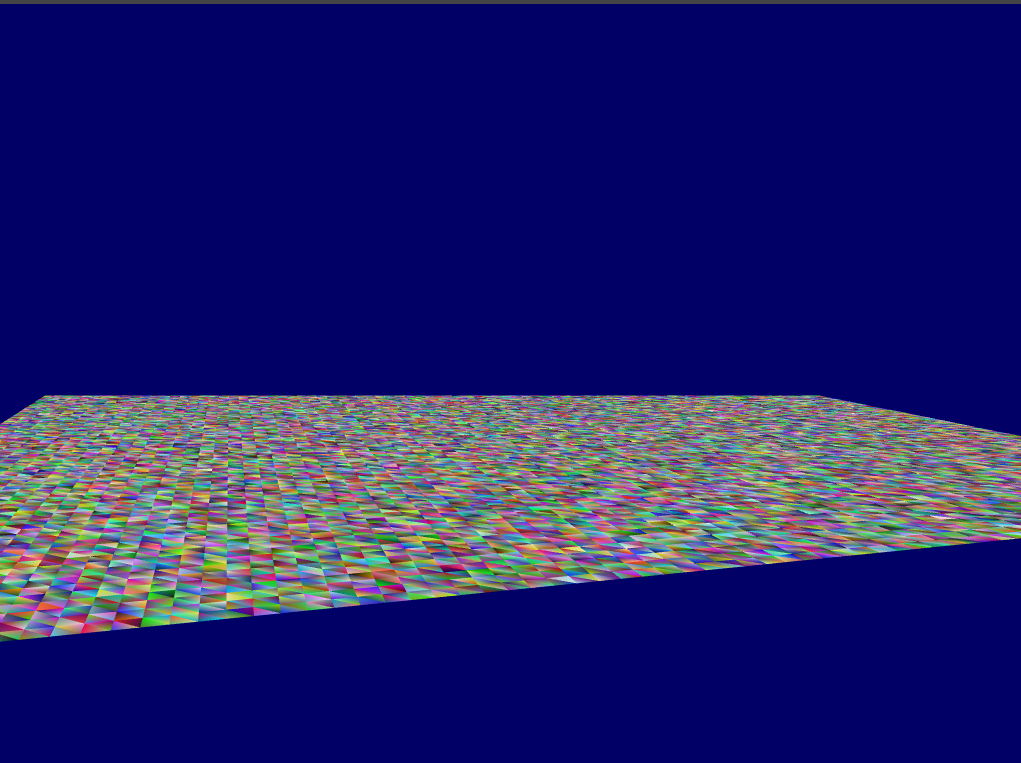
\includegraphics[width=.9\linewidth]{Images/Sprint-Images/Sprint3-2.png}
  \captionof{figure}{Generation of a flat plane}
  \label{fig:sprint3-2}
\end{minipage}%
\begin{minipage}{.5\textwidth}
  \centering
  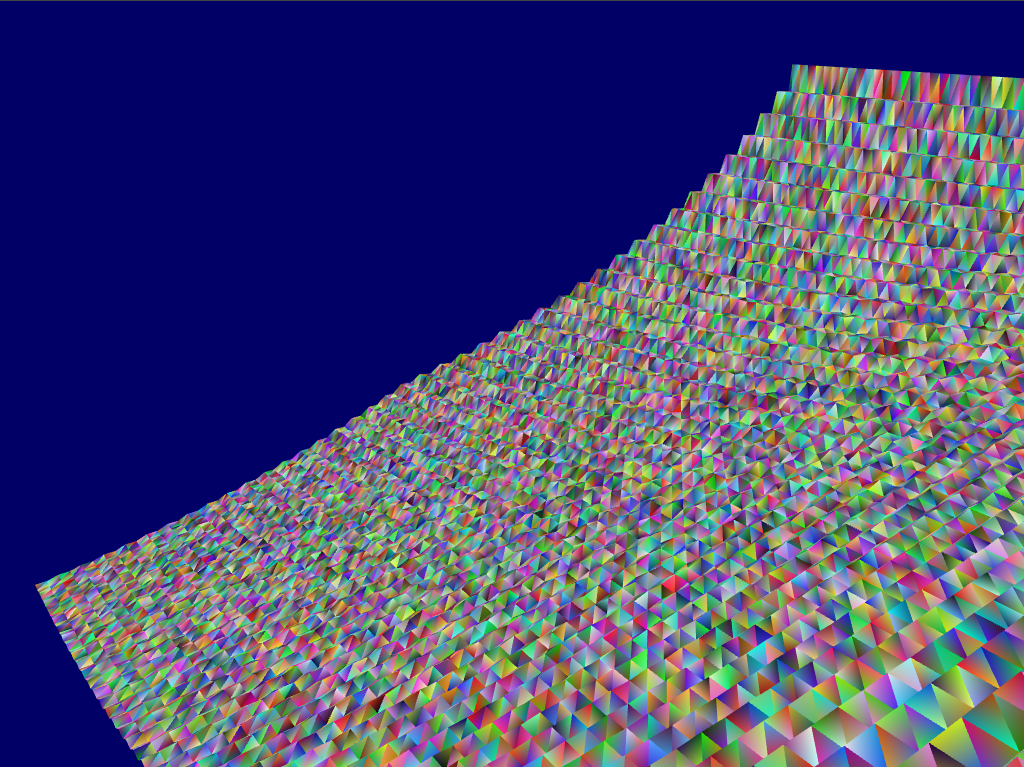
\includegraphics[width=.9\linewidth]{Images/Sprint-Images/Sprint3-3.png}
  \captionof{figure}{Initial output of the broken Diamond Square algorithm}
  \label{fig:sprint3-3}
\end{minipage}
\end{figure}

\subsection{Sprint Goals}
\begin{enumerate}
    \item \textit{As the Developer, I need to continue working on my Diamond Square Algorithm - fixing the algorithm itself and using the heightmap to generate a grid, so that I can have usable terrain. }
\end{enumerate}
\subsection{Sprint Summary}
The third sprint's main aim was to continue to improve on the Diamond Square Algorithm, and perform small tweaks on the rest of the code. This was achieved by successfully interpreting a heightmap into vertices, as well as continued iteration over the Diamond Square algorithm in order to bring it to a successful implementation state. Personally, this week was very busy, and so not as much work could be achieved in comparison to other Sprints. \medskip

A significant accomplishment of this sprint was both implementing the Camera's movement, as well as generating a flat plane, before applying the heightmap to the plane. This was buckets ahead of the previous week, and gave ample motivation to keep pressing ahead to make the Diamond Square algorithm work. 

\clearpage
\section{Sprint 4 (05/03/18 - 11/03/18)}

\begin{figure}[h!]
    \centering
  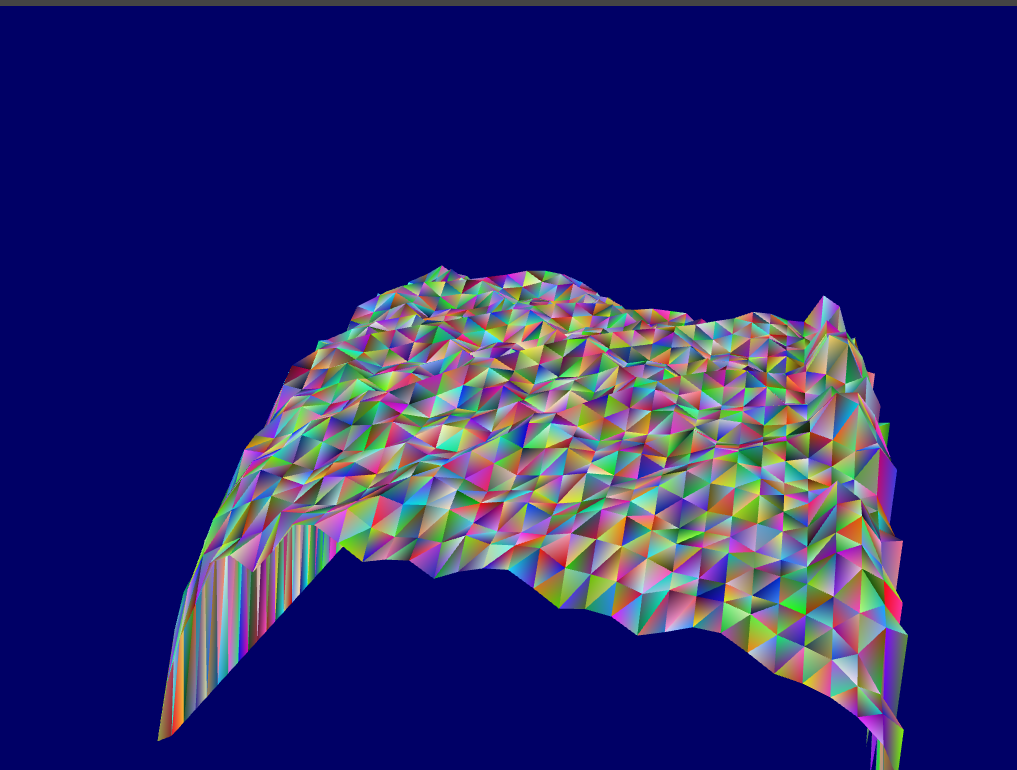
\includegraphics[width=0.5\textwidth]{Images/Sprint-Images/Sprint4-7.png}
 \caption{Final state of the Diamond Square terrain by the end of the Sprint}
 \label{fig:sprint4-1}
\end{figure}

\subsection{Sprint Goals}
\begin{enumerate}
    \item \textit{As the Developer I need to fix/re implement the Diamond Square algorithm so that it generates suitably random terrain, so that I can begin to implement details and have something impressive for my Mid Project Demonstration. }
    \item \textit{As the Developer, I want to implement some code to make colour based on the height of the vertex, so that the terrain is not simply random colours.}
    \item \textit{As the Developer, I want to increase the size and scalability of the Heightmap Implementation, allowing for more vertices to be displayed on screen, whilst shrinking the current vertices. }
    \item \textit{As a student, I want to make a poster highlighting my project, in order to submit it for CS38220.}
    \item \textit{As a student I need to begin to prepare for my mid project demonstration, in order to be able to present something of high enough quality. }
    
\end{enumerate}
\subsection{Sprint Summary}

The fourth sprint's main aim was to bring the Diamond Square Algorithm to a stage where it generated suitable terrain, as well as beginning to implement colour vertex code. The week also coincided with creation of a poster detailing the project, for a separate module. This was achieved by even more iteration on the Diamond Square algorithm, adjusting it to allow for it to output larger vertex buffers. Colour Vertex Buffers were begun to be worked on, but required more time than initially scoped for, due to syntax issues and the implementation being more complicated than initially thought.  \medskip

A significant accomplishment during this sprint was managing to get the code to output vertices that began to take the correct form - becoming more \textit{terrain-like} in nature (see fig~\ref{fig:sprint4-1}) , instead of one long curve (see fig~\ref{fig:sprint3-3}), as in the previous sprint. 

\clearpage

\section{Sprint 5 (12/03/18 - 18/03/18)}

\begin{figure}[h!]
\centering
\begin{minipage}{.5\textwidth}
  \centering
  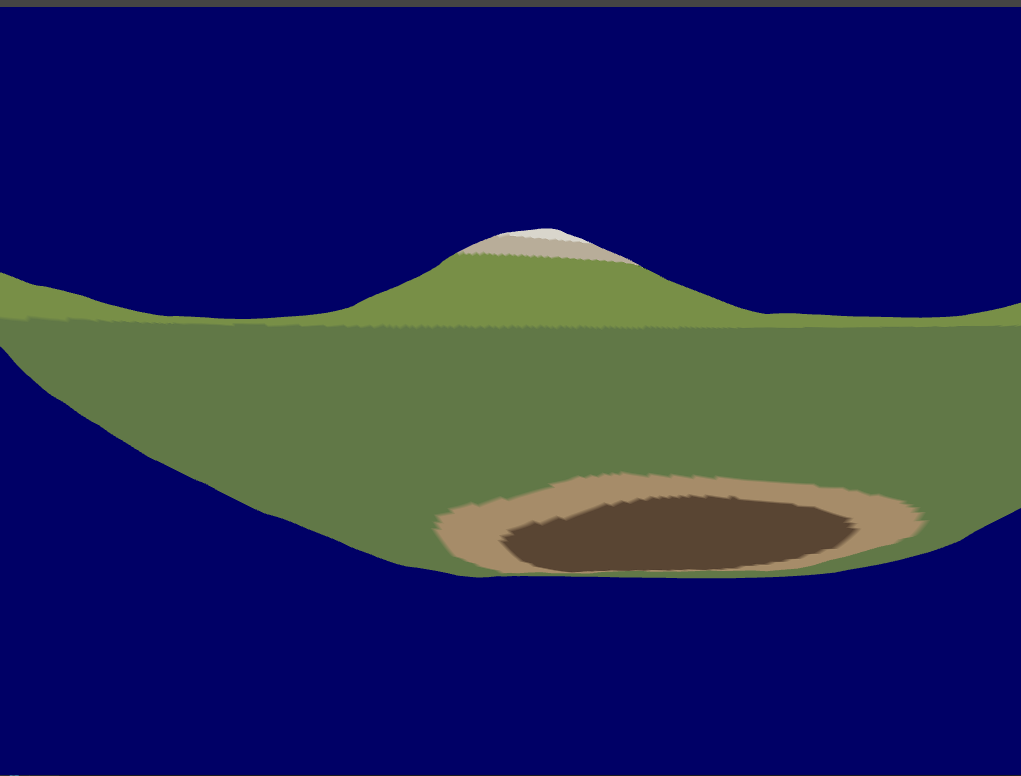
\includegraphics[width=.9\linewidth]{Images/Sprint-Images/Sprint5-3.png}
  \captionof{figure}{Initial terrain generation}
  \label{fig:sprint5-3}
\end{minipage}%
\begin{minipage}{.5\textwidth}
  \centering
  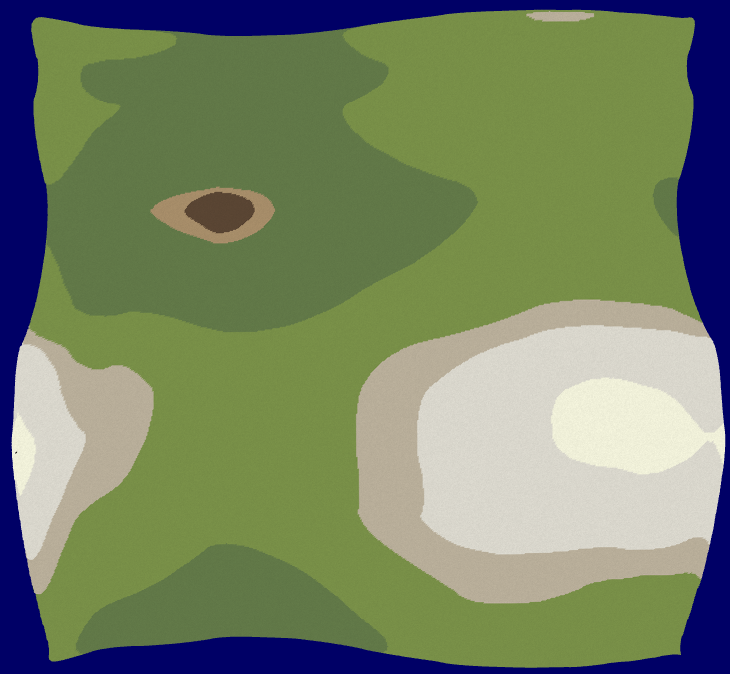
\includegraphics[width=.9\linewidth]{Images/Sprint-Images/Sprint5-6.png}
  \captionof{figure}{Top down view of the terrain}
  \label{fig:sprint5-6}
\end{minipage}
\end{figure}


\subsection{Sprint Goals}

\begin{enumerate}
    \item \textit{As a developer, I need to continue to look at the Diamond Square Algorithm and fully fix it this week - it is very nearly fixed, but continues to need tweaking. It would be good to have it working fully for my mid project demo. }
    \item \textit{As a student, I need to continue work on my report, so that I don't fall too far behind overall.}
    \item \textit{As the Developer, I want to increase the size and scalability of the Heightmap Implementation, allowing for more vertices to be displayed on screen, whilst shrinking the current vertices. }
    \item \textit{As a developer, I'd like to add some basic colours to the heightmap, to make it look more natural.}
    \item \textit{As a student, I need to finish prepping for my mid project demo, so that I can demo it well to my 2nd marker. }
    
\end{enumerate}
\subsection{Sprint Summary}

The fifth sprint's main aim was to finish work on the Diamond Square algorithm, which included vertices generated, size of grid and colour of grid. This was achieved through solving the final bugs in the Diamond Square algorithm, implementing multiple arrays defined by the size of the grid given to the method and a method which sets a vertex colour depending on its height. This was one of the most rewarding sprints of the entire project, as the terrain went from a glitchy multicoloured mess, to a cohesive plane, which was recognisable as terrain. This sprint was the last sprint allocated for work on the Diamond Square algorithm, as otherwise there would be not enough time left to work on other aspects of the project, so successfully implementing the terrain was a big relief. \medskip

A significant accomplishment during this sprint was implementing colour into the terrain. As this project is graphics based, what appears onscreen is what matters most, so in implementing both colour and terrain in one sprint, the project's quality was lifted significantly.

\clearpage

\section{Sprint 6 (19/03/18 - 26/03/18)}


\begin{figure}[h!]
\centering
\begin{minipage}{.5\textwidth}
  \centering
  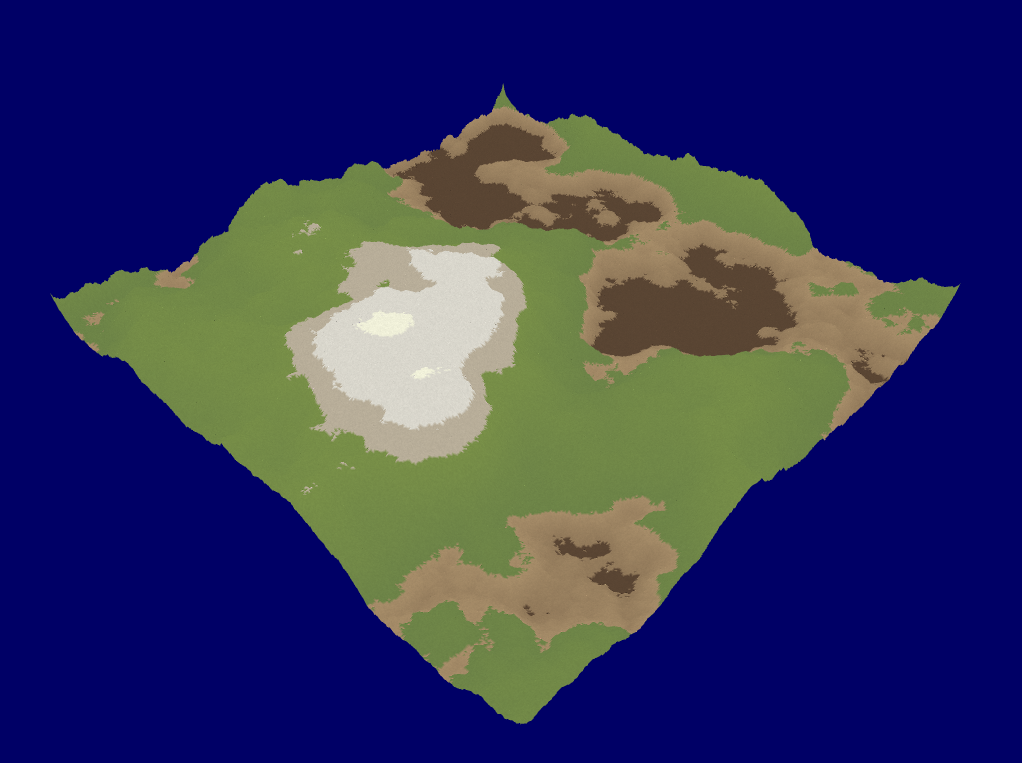
\includegraphics[width=.9\linewidth]{Images/Sprint-Images/Sprint-7-After-Colour.png}
    \captionsetup{width=.9\linewidth}
  \captionof{figure}{Edited Diamond Square, with blended colours}
  \label{fig:sprint7-c}
\end{minipage}%
\begin{minipage}{.5\textwidth}
  \centering
  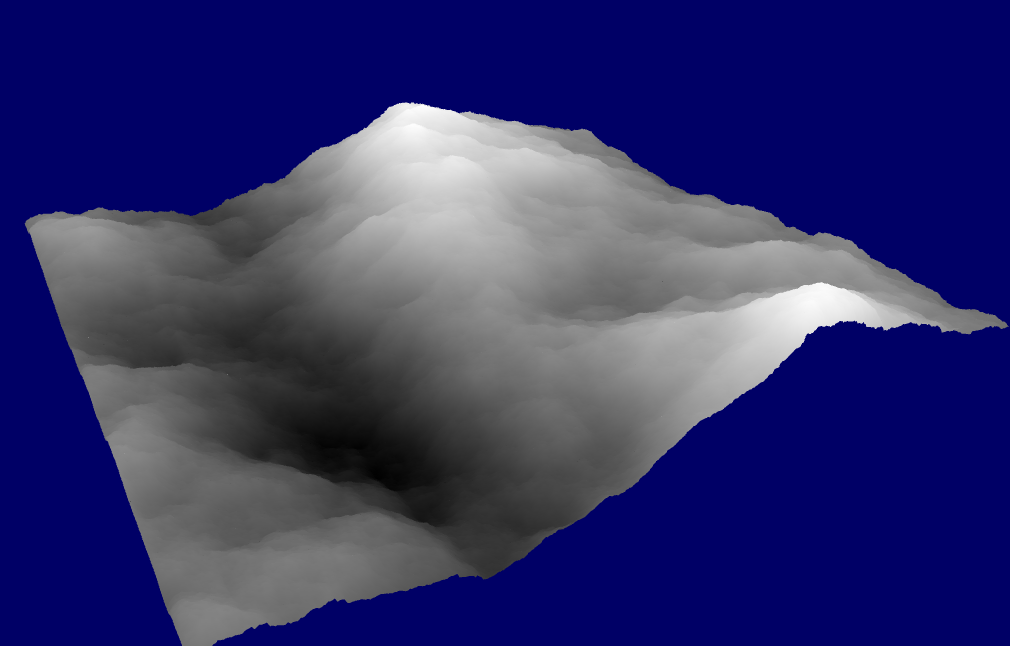
\includegraphics[width=.9\linewidth]{Images/Sprint-Images/Sprint-7-After-Greyscale.png}
    \captionsetup{width=.9\linewidth}
  \captionof{figure}{Diamond Square with a greyscale texture mapped to it (the higher the terrain, the lighter the colour)}
  \label{fig:sprint7-g}
\end{minipage}
\end{figure}

\subsection{Sprint Goals}

\begin{enumerate}
    \item \textit{As a developer, I need to begin to implement L-System trees, so that I can begin to look past simple implementation and move onto rendering optimisation.  }
    \item \textit{As a developer, I need to fix triangle culling, so that I can half the amount of triangles rendered and increase the frame rate of the program.}
    \item \textit{As a student, I need to write a lot more report to ensure that I am not falling behind. }
    \item \textit{This week also has a deadline for professional issues, which will interfere with my work for the major project.}
    
\end{enumerate}
\subsection{Sprint Summary}

The sixth sprint's main aim is to research and subsequently begin implementation of L-Systems, as well as fixing small issues, such as face culling and a blended colour implementation. This was achieved by a lot of L-System research, before initial implementation of a class and method to build the initial string, a well as a quick rewrite of the order the vertices were pushed to the Vertex Buffer in order to enable face culling and blending colours by getting a percentage in between two shades and applying this to the terrain to create a gradient, rather than a block of colour. \medskip

This sprint clashed with another module's assignment deadline, as well as the end of second semester, meaning that a day was lost to moving back home. However, in the last few minutes of the sprint, a change was made to Diamond Square which made the terrain a lot more detailed, instead of a smooth curve, the project gained a lot more of a realistic look. \medskip

A significant achievement during this sprint was fully understanding L-Systems. A lot of the initial research was focused on terrain generation and OpenGL syntax, so finding time to understand and begin to implement L-Systems meant that implementation would be better prepared for the coming sprints. \clearpage
\section{Sprint 7 (26/03/18 -  01/04/18)}

\subsection{Sprint Goals}

\begin{enumerate}

\item \textit{As a developer, I need to get L-Systems to an initial state of being rendered, so that I can focus on improving them and where they are placed.}

\item \textit{As a developer, I need to refactor the design of my code so that it is better structured and easier to maintain.}

\item \textit{As a student, I need to add a lot more to my report. }
\end{enumerate}

\subsection{Sprint Summary}

The seventh sprint's primary aim was to focus more on the write up of the project, as well as to prepare and begin implementation of L-Systems. This was achieved by researching GLM (OpenGL Mathematics)~\cite{creation2016opengl}, reading up more on L-System implementation~\cite{prusinkiewicz2012algorithmic} and beginning to implement the algorithms needed for L-Systems.\\

A significant achievement during this sprint was getting a significant chunk of the report written - at this stage of the project the report should be eating into development time more and more.


\section{Sprint 8 (02/04/18 -  08/04/18)}


\begin{figure}[h!]
\centering
\begin{minipage}{.3\textwidth}
  \centering
  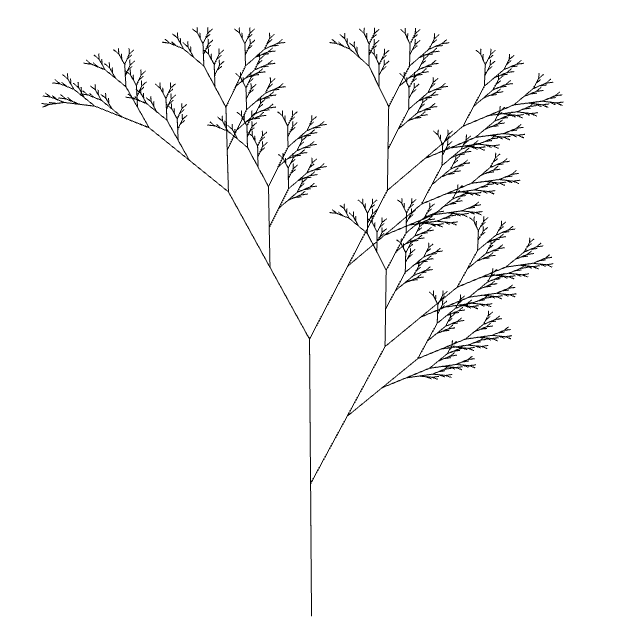
\includegraphics[width=.9\linewidth]{Images/Sprint-Images/tree1.png}
    \end{minipage}%
\begin{minipage}{.3\textwidth}
  \centering
  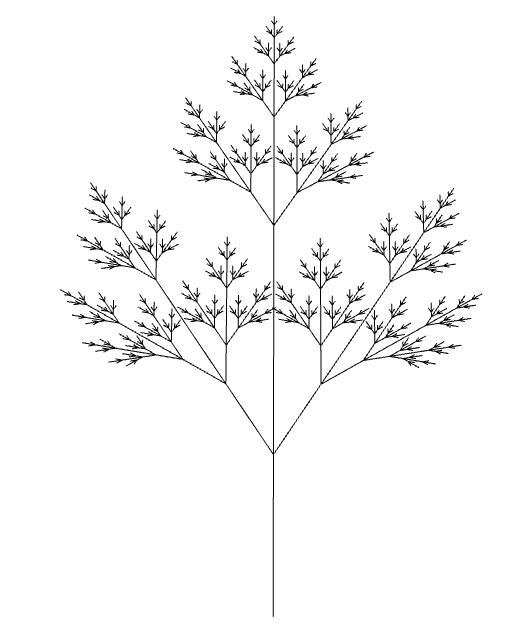
\includegraphics[width=.9\linewidth]{Images/Sprint-Images/tree2.png}
\end{minipage}
\begin{minipage}{.3\textwidth}
  \centering
  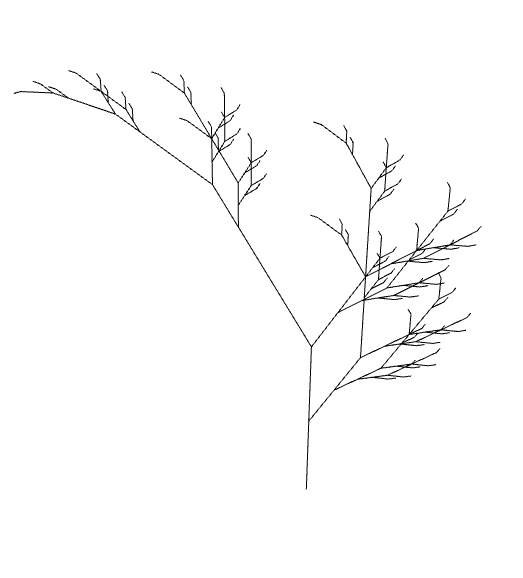
\includegraphics[width=.9\linewidth]{Images/Sprint-Images/tree3.png}
\end{minipage}
\caption{Three examples of 2D trees generated using L-Systems}
 \label{fig:sprint8}

\end{figure}
\begin{enumerate}
\subsection{Sprint Goals}

\item \textit{As a developer, I want to finish L-systems so I can get onto optimisations and restructuring the program as a hole.}

\item \textit{As a student, I want to start my second section of my report, whilst also redrafting my first section.}
\end{enumerate}

\subsection{Sprint Summary}

The eighth sprint's main aim was to fully implement L-Systems, as well as begin section two of the report. This will be achieved by implementing the rest of the L-System code, started in Sprint Seven. The trees were initially implemented using 2D maths, following examples in The Algorithmic Beauty of Plants~\cite{prusinkiewicz2012algorithmic}. The option to move the camera with WASD as well as the arrow keys was also added during this sprint. On top of this, code was cleaned up and restructured, a lot of world generation code moving into the World Maker class.

A significant achievement in this sprint was getting 2D L-Systems working (see fig~\ref{fig:sprint8}, meaning that the two key components to the project - terrain and trees are technically in. 


\clearpage
\section{Sprint 9 (09/04/18 -  15/04/18)}

\begin{figure}[h!]
    \centering
  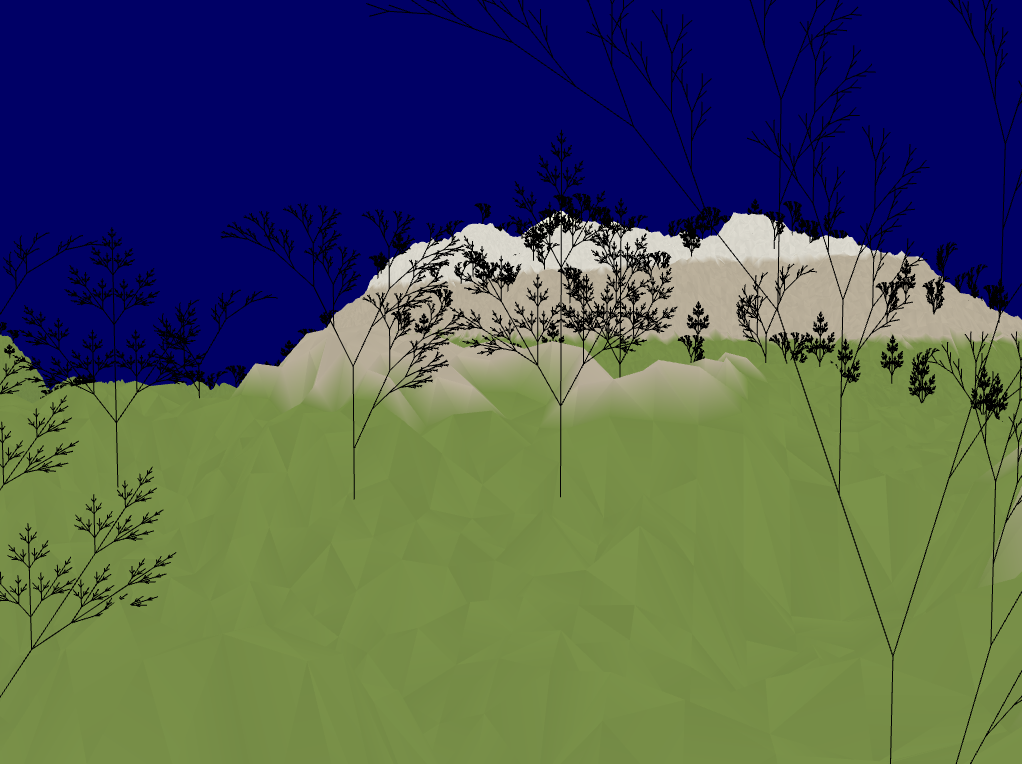
\includegraphics[width=0.5\textwidth]{Images/Sprint-Images/Sprint9-1.png}
 \caption{An example of instance rendering - only one copy of the each of the three models of trees is stored.}
 \label{fig:sprint9-1}
\end{figure}

\subsection{Sprint Goals}
\begin{enumerate}
    \item \textit{ As a developer, I am going to work on placing L-System objects, in order to create a dense scene.}

    \item \textit{ As a developer, I am going to look at and implement instance rendering for my L-System objects, in order to keep render time relatively low.}

    \item \textit{ As a developer, I am going to look at Level Of Detail and Billboarding, so that I can keep render time low.}

    \item \textit{ As a developer I am going to begin to look at my UI and how I can improve the current User Experience with my project.}

    \item \textit{ As a student, I want to start my second section of my report, whilst also redrafting my first section. }
\end{enumerate}


\subsection{Sprint Summary}

The ninth sprint was focused on implementing instance rendering, and redesigning the Diamond Square algorithm to store all of its generations, in order to then implement them with Level Of Detail optimisations. As well as this, the report was continually worked on. This was achieved by implementing instance rendering, alongside a basic tree placement method, as well as redesigning the Diamond Square class so that it saved each iteration it generated in a Vector. \medskip

A significant accomplishment this sprint was getting instance rendering working (see fig~\ref{fig:sprint9-1}. Instance rendering is a form of the Flyweight Design Pattern, and saves hugely on memory.

\clearpage
\section{Sprint 10 (16/04/18 -  22/04/18)}

\begin{figure}[h!]
\centering
\begin{minipage}{.3\textwidth}
  \centering
  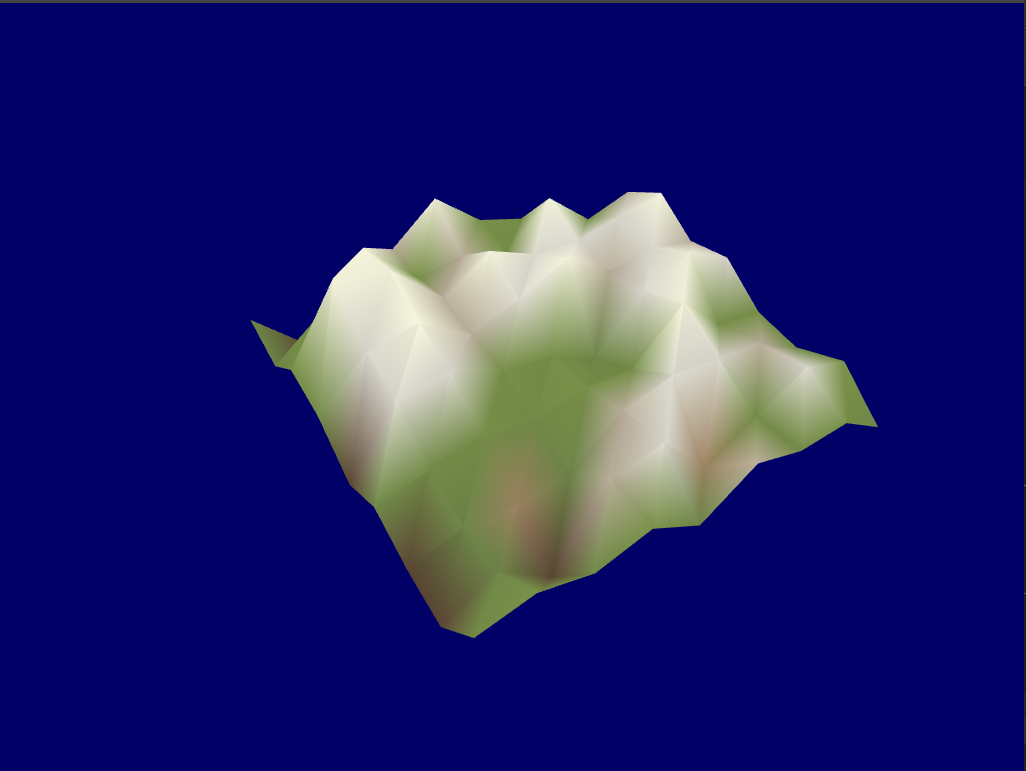
\includegraphics[width=.9\linewidth]{Images/Sprint-Images/Sprint10-1.png}
    \end{minipage}%
\begin{minipage}{.3\textwidth}
  \centering
  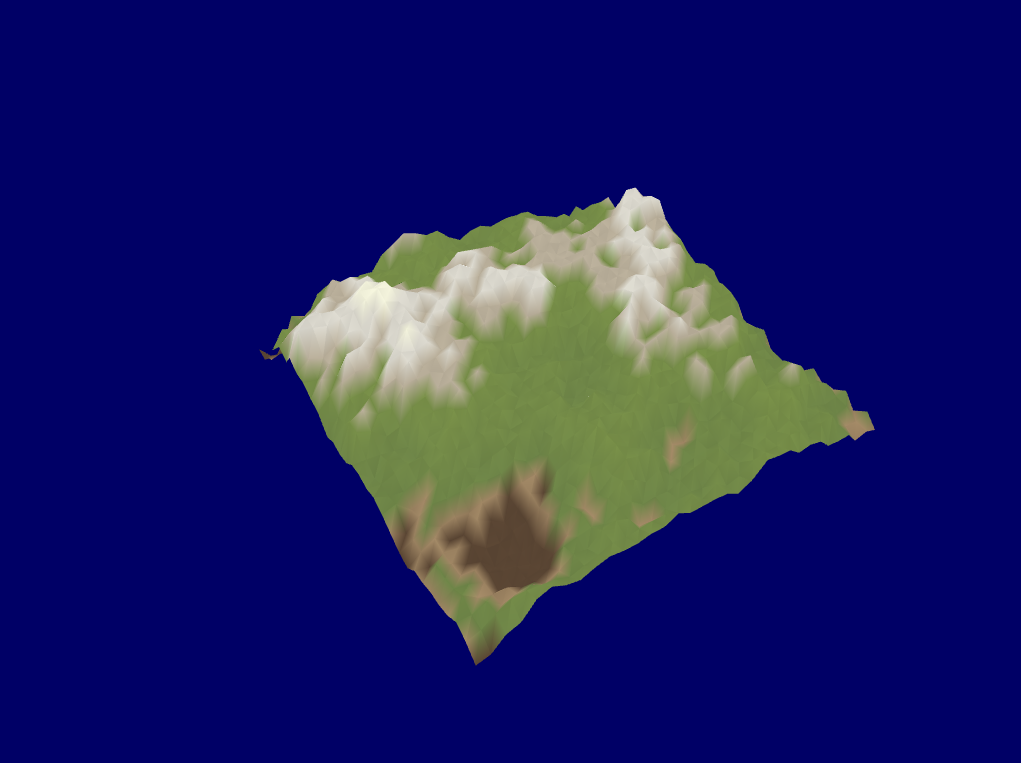
\includegraphics[width=.9\linewidth]{Images/Sprint-Images/Sprint10-2.png}
\end{minipage}
\begin{minipage}{.3\textwidth}
  \centering
  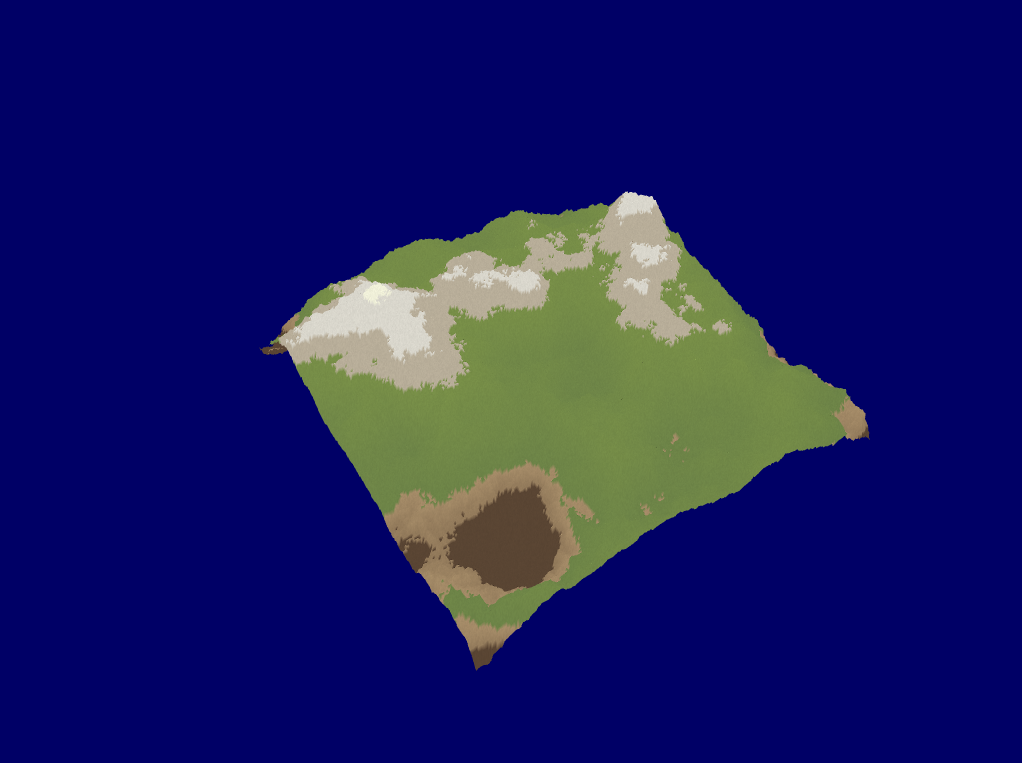
\includegraphics[width=.9\linewidth]{Images/Sprint-Images/Sprint10-3.png}
\end{minipage}
\caption{Three different Levels Of Detail of Terrain}
\label{loddiamondsq}
\end{figure}
\subsection{Sprint Goals}

\begin{enumerate}

    \item \textit{As a developer I want to further implement Level Of Detail for terrain, drastically cutting down on the amount of vertices rendered.}

    \item \textit{As a developer I am going to begin to look at my UI and how I can improve the current User Experience with my project.}

    \item \textit{As a developer, I am going to begin to implement unit tests into my code, in order to create a more robust program. }
    \item \textit{As a Student I want to add at least 2000+ more words to my report.}

\end{enumerate}

\subsection{Sprint Summary}

The tenth sprint's main aim was to add in Level Of Detail optimisations for terrain, look at implementing some UI and Unit Tests and do a lot of report work. Unit tests were implemented using Boost~\cite{boost}, UI was considered with NanoGUI~\cite{nanogui}. The most work was done on continuing to implement Quadtree Level Of Detail tessellation, continuing to adapt the Diamond Square class to store all of its iterations. \medskip

A significant accomplishment during this sprint was reworking the entire Diamond Square class to store all iterations. This prepares the project for the implementation of Quadtrees in the following sprint. Getting Unit Tests up and going for the project was also a good achievement, as ensuring that everything is working by the end of the project is useful.


\clearpage
\section{Sprint 11 (23/04/18 -  29/04/18)}

\subsection{Sprint Goals}
\begin{enumerate}
    \item\textit{ As a developer I want to further implement Level Of Detail for terrain, drastically cutting down on the amount of vertices rendered.}

\item\textit{ As a developer I am going to begin to look at my UI and how I can improve the current User Experience with my project.}

\item\textit{ As a developer, I am going to continue to implement unit tests into my code, in order to create a more robust program. }

\item\textit{ As a developer, I want to have one more go at attempting to make my trees 3D. }

\item\textit{ As a Student I want to add at least 2000+ more words to my report.}

\end{enumerate}

\subsection{Sprint Summary}
Sprint Eleven's main aims were to tie up all loose ends in terms of programming, whilst finding time to continue to contribute to the report. This was achieved through getting a working version of Quadtree Level Of Detail optimisation (albeit one that had a negative effect on the frame rate rather than a positive one), more unit tests being implemented and more words being written. Quaternions were also used to replace the 2D maths in the L-Systems, but it was not sufficient enough progress to get 3D trees to work. \medskip

A significant accomplishment during this sprint was getting Quadtrees to work as intended.

\section{Post Sprint Progress}
The sprints were planned to finish to give me five days to focus on completing the report and chasing up any loose ends (such as further unit tests). A couple more features were also added to the project, in order to ensure that the final demo of the project goes smoothly. These were mainly keyboard shortcuts to perform the following actions:

\begin{itemize}
    \item Displaying and hiding the terrain
    \item Displaying and hiding the L-Systems
    \item Selecting a Level Of Detail to display
    \item Selecting a colour palette to display
\end{itemize}

\chapter{Tests}
\section{Testing Methodology}
The testing on this project was carried out through a mix of Unit and Manual testing. This approach was chosen as this project is procedural. This means that results differ each time, meaning that it is hard to test effectively through unit tests alone. Therefore manual testing is required in order to ensure that the project is working as fully intended.

\subsection{Unit Tests}
\subsubsection{Diamond Square Unit Tests}

The Unit tests for the Diamond Square class ensure that the height map and vertex generation functions work correctly, by checking the size and content of the vectors generated. 

\subsection{Manual Tests}

\subsection{User Input}

As a lot of the usability of the project is based on User Input, there have been manual tests performed to ensure that the project is working as intended. These have included checking that every intended input for the user works. The current input into the project controls the Level Of Detail displayed on screen, whether the terrain or l-systems are displayed, what colour the terrain is displayed in, and camera movement.

\subsection{Vertices Displayed}

These manual tests were to ensure that the vertices displayed on screen did not have any significant graphical glitches, and the terrain and trees were generated and distributed randomly each program iteration.

\chapter{Implementation Results}
\section{Problems Faced}
\subsection{Diamond Square}

\begin{figure}[h!]
    \centering
  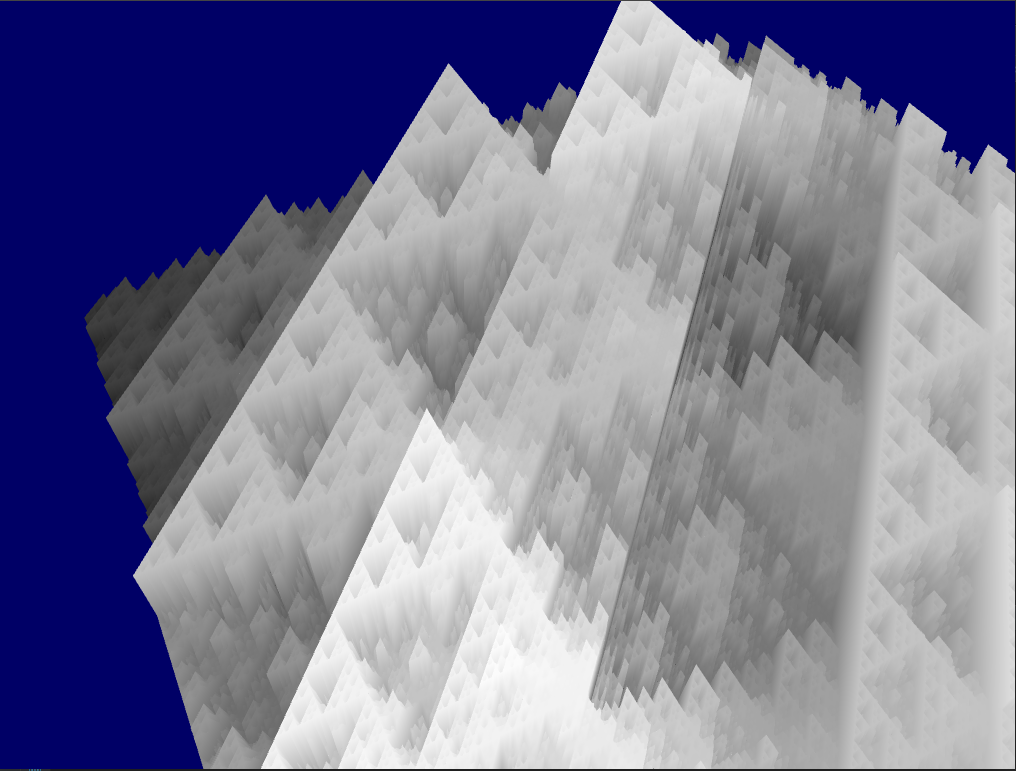
\includegraphics[width=0.4\textwidth]{Images/Screenshots/Glitch.png}
 \caption{The appearance of terrain if the Square and Diamond steps are swapped}
 \label{fig:glitch}
\end{figure}

Diamond Square Generation was the class which had most time spent on it, due to a mixture of it being early on in the report and having not much documentation of it online. Due to the early nature of its implementation, less OpenGL and C++ syntax was known, which meant that more bugs were likely. The main issue with the algorithm was over complicating it. When initially implementing it, the solution was messy and inelegant, compared to the final diamond square loop (see fig~\ref{fig:diamondsquareimpl}). Confusion over the naming conventions of Diamond and Square meant that they were initially implemented the wrong way round, causing patterns such as fig~\ref{fig:glitch} to manifest. \medskip
\clearpage

\begin{figure}[h!]
\centering
\begin{minipage}{.4\textwidth}
  \centering
  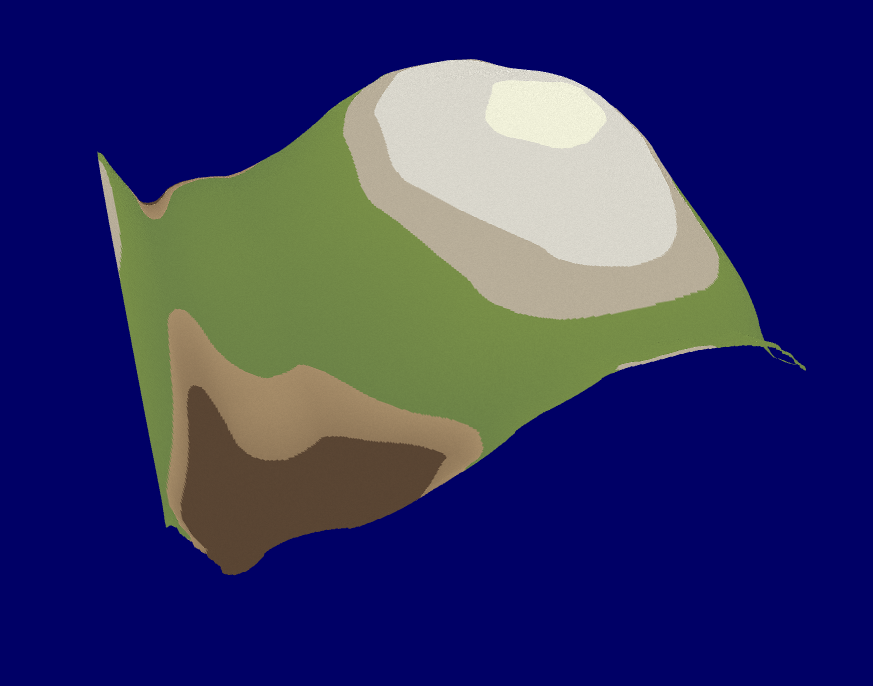
\includegraphics[width=.9\linewidth]{Images/Sprint-Images/Sprint-7-Before-Colour.png}
    \end{minipage}%
\begin{minipage}{.4\textwidth}
  \centering
  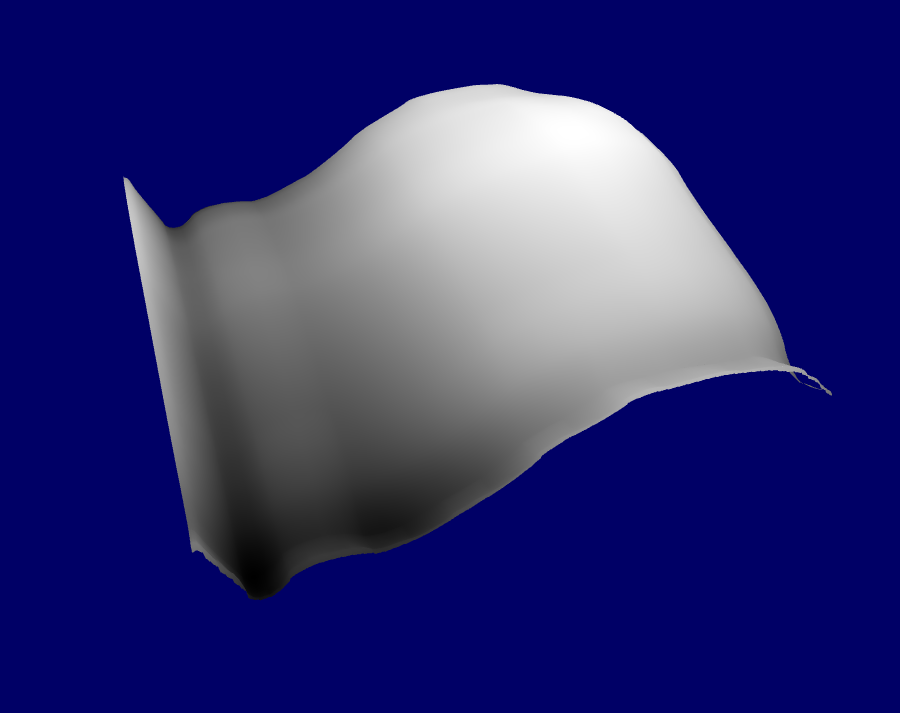
\includegraphics[width=.9\linewidth]{Images/Sprint-Images/Sprint-7-Before-Greyscale.png}
\end{minipage}
\caption{Before the randomness factor was changed}
\label{before-random}
\end{figure}


\begin{figure}[h!]
\centering
\begin{minipage}{.4\textwidth}
  \centering
  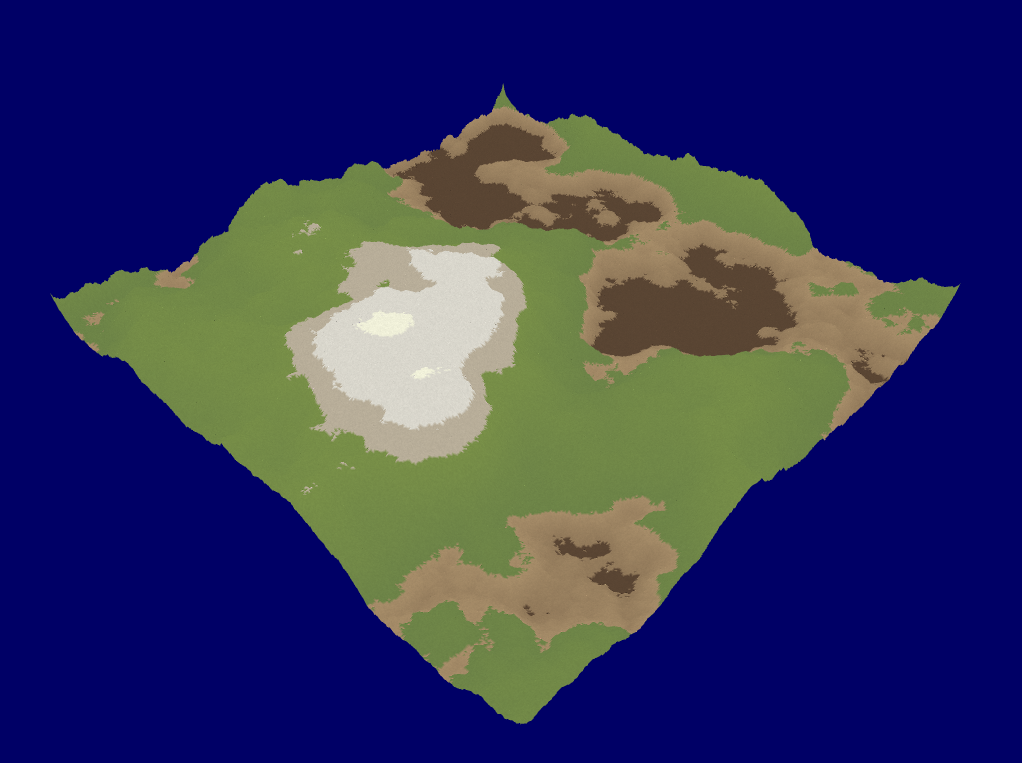
\includegraphics[width=.9\linewidth]{Images/Sprint-Images/Sprint-7-After-Colour.png}
\end{minipage}
\begin{minipage}{.4\textwidth}
  \centering
  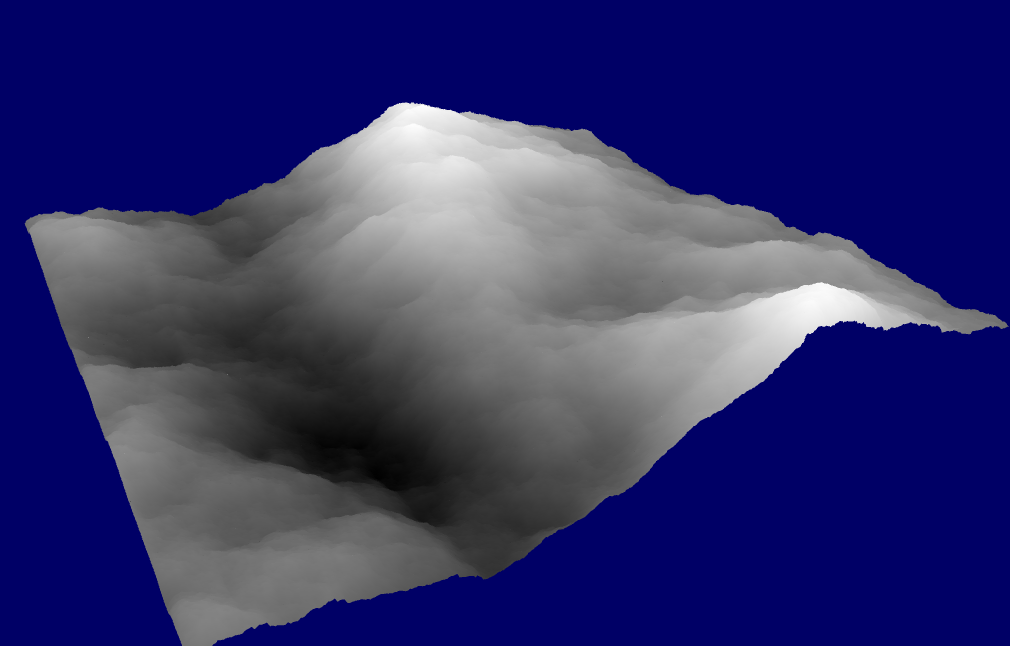
\includegraphics[width=.9\linewidth]{Images/Sprint-Images/Sprint-7-After-Greyscale.png}
\end{minipage}
\caption{After the randomness factor was changed}
\label{after-random}
\end{figure}


As well as this the terrain initially began very smooth - which was not originally seen as an issue until it was accidentally solved. The issue was that the random height variable was only updated each iteration, rather than every diamond and square step. Due to this, randomness of terrain was severely reduced, until the randomly generated offset number was refreshed each step. The effects of this change can be seen in fig~\ref{before-random} and fig~\ref{after-random}.

\begin{figure}[h!]
    \centering
  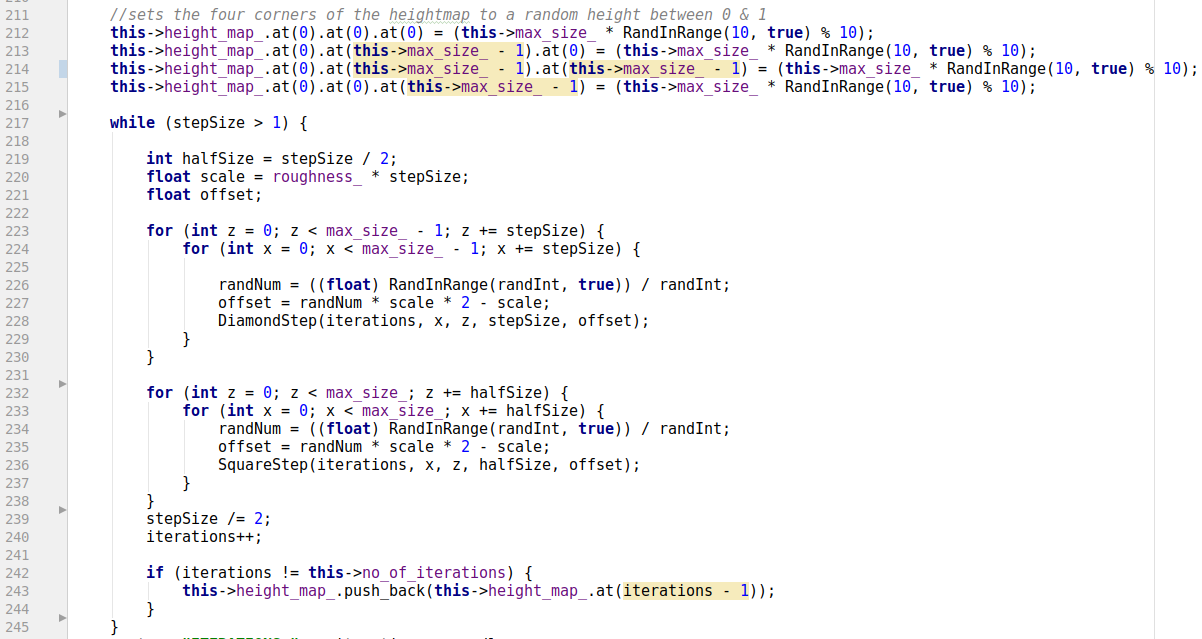
\includegraphics[width=0.8\textwidth]{Images/Code-Snippets/DiamondSquareAlgorithm.png}
 \caption{The final implementation of the Diamond Square algorithm}
 \label{fig:diamondsquareimpl}
\end{figure}

\subsection{L-Systems}

Perhaps the largest issue encountered during L-Systems was when implementing them with 2D maths instead of 3D maths was a loss of precision in angles. If a fractal string's rotations in an axis are only in  one direction then a loss of precision happens due ever increasing numbers. This was solved by limiting the angles to numbers in the 0-360 range.

\subsection{Terrain Quadtree}

The biggest problem when approaching the implementation of Quadtrees for the terrain was the question of how to generate lower level of detail representations of the terrain. This problem was quickly solved when the realisation came that the Diamond Square algorithm essentially generates a new Level of Detail for the terrain each iteration (see fig~\ref{loddiamondsq}), as it is a fractal based terrain height map generator. 

\subsection{Colour Palette}
When the initial colour palette was implemented, the entire terrain was filled with flat colour, causing depth perception to be a little unreliable. This was because when looking into the distance, it was hard to find distinguishing features for your eye to latch onto. This was solved by varying the colour on each triangle by a couple shades. This gave the terrain a more stylistically pleasing look, whilst also solving the problem of a lack of depth perception. 

\section{Unresolved Problems}
\subsection{3D Trees}
3D trees are still not implemented into the project. During implementation, applying the core concepts of 3D maths to the syntax of GLM, and then translating that into 3D Vertices which OpenGL would be able to interpret proved a difficult struggle. Steps were made towards the goal of 3D trees - Quaternions eventually replaced the initial implementation of 2D maths, but the project ran out of development time before the problem could be solved.

\subsection{Level Of Detail Quadtree Tessellation}
This was another aim of the goal that remained incomplete due to the lack of time. Whilst the basic implementation is within the code, it fell foul to implementation choices made earlier on in the project, when C++ syntax was less known. Quadtree implementation works by initially creating a quadtree of the size 1x1, dividing the subsections into boundarys smaller than one. Theoretically, this quadtree can then simply be taken and applied to the vertices generated by the Diamond Square class. However, DiamondSquare takes in multiple arrays in order to store high amounts of vertices as the program segfaulted if only one array was used. These array store the vertices in the format of one long array. Due to this awkward storage solution, and the fact that quadtrees were being implemented so close to the end of the project, the quickest solution was to reuse code which interpreted the initial heightmap as vertices. This proved wildly inefficient and instead of seeing a framerate uptick, instead the program essentially ground to a halt, averaging less than 1 frame per second. \medskip

A solution to this problem would be to rework the DiamondSquare vertice generator (and subsequently everything which uses its output format) into using a single vector. This vector would be a lot more usable and provide an easier way to access the vertices once generated. However, due to the amount of methods which work around the format of which DiamondSquare currently outputs, there was not enough time left in the project to rework the method. \medskip

A second problem with this algorithm is the placement of objects on the terrain. Each object is placed on the terrain in regards to the final Level Of Detail - when the Level Of Detail changes, the object is often submerged inside of the bigger triangle which replaces it. In order to not recalculate the position of every single object each frame, the position of every static object for each level of detail would have to be worked out in the setup stages of the project, adding a longer initialisation time to the project. 

\section{Potential Future Additions}

On top of the issues listed in the previous subsection, there are a myriad of potential future additions that could be added to this project. 

\subsection{Optimisation}
The most pressing issue before adding anything else would be more optimisations. The project didn't have time to begin to implement L-System optimisations, which would be the immediate optimisation. As well as this, the code called in the draw loop would be assessed to try to decrease the render time per frame.  

\subsection{L-Systems}
At the moment, L-Systems are simply drawn with lines - something which detracts from the project's overall aesthetic. Drawing them using a 3D primitive such as a cylinder would be a good start to improving the overall feel of them, as well as creating a more impressive scene visually. 

\subsection{UI}

UI was initially planned for the project, but again abandoned due to lack of time. However, the library NanoGUI~\cite{nanogui} is a UI widget library with easy OpenGL integration, which could be used to display a simply UI to control the scene with, instead of keyboard commands. The keyboard commands show the simplicity of how the scene can be controlled, so UI integration is  a viable option.

\subsection{Physics}

Physics added into the project would be a useful way of adding more fun interactions into the world, turning it from simply a graphics visualiser and beginning to move it more into game territory. This could be implemented using Bullet~\cite{coumans2013bullet}, a popular physics library for OpenGL. 

\subsection{Different Algorithms}
An interesting direction to go in the future of this project is using it as a comparison tool for procedurally generated algorithms. It could potentially be used to easily see the different type of terrain each algorithm produces, as well as easy performance comparisons. 

\subsection{More Content}
The  most obvious, is more content. At the moment, the project only has l-systems and terrain implemented. Integrating more content is a quick way to make the project feel more alive and of higher quality (to a certain extent). Moving animals, grass and flowers, trees swaying in the wind or shedding leaves (using a particle system) are all more content which could be added.

\chapter{Conclusion and Evaluation}
\section{Evaluation}

\subsection{Project Aims}
\subsection{Create a 3D Procedurally Generated Nature Scene}
The first aim of this project was to create a 3D procedurally generated nature scene. The basic aim was to implement Terrain and Trees as an initial goal - one that has been achieved. The project generates a scene which is different each time, with procedural terrain and procedural trees with an algorithm which places them in random positions each iteration. \medskip

However, the scene is still quite basic, mainly due to the current L-System implementation. Trees are still represented in 2D with black lines, which clash with the landscape. With only trees on the landscape, it also tends to lose a sense of scale. However, the initial aim was to implement two to three procedural generation algorithms, and that aim has been met, with the implementation of both Diamond Square terrain and Lindenmayer Systems. 

\subsection{Become competent with C++, OpenGL and the core fundamentals of low level graphics}

The second aim of the project is one is more fulfilled than the first. The project demonstrates a confidence with the core fundamentals of low level graphics, C++, and OpenGL. At the beginning of the project, there was only a vague familiarity with C++, in comparison to the end of the project, where a complex program such as this has been built.  There is still a lot more knowledge to be learnt - namely the intricacies of OpenGL and C++, but overall this aim has been comfortably reached.

    
\clearpage

\appendix

\chapter{Third Party Code and Libraries}

\section{Classes \& Functions}

When creating the project, the tutorials found on http://opengl-tutorial.org~\cite{opengl_tutorial} were followed. Some of the code used within those tutorials was reused in this project, with permission under the WTFPL Public Licence~\cite{wtfpl}. \medskip

\textit{\textbf{shader.cpp}}, \textit{\textbf{ColorFragmentShader.fragmentshader}} and \textit{\textbf{TransformVertexShader.vertexshader}} remain unchanged when compared with tutorial code. \medskip

\textit{\textbf{l\_system\_colour.frag.glsl}} and \textit{\textbf{l\_system\_transform.vert.glsl}} were written independently, but with guidance from previous tutorial files.\medskip

\textit{\textbf{controls.cpp}} and \textit{\textbf{main.cpp}}) began initially as code simply taken from the tutorial, but both have had extensive reworks and changes, when compared to the initial code provided by the tutorial. Specifically, whilst the methods \textit{\textbf{computeMatricesFromInputs()}}, \textit{\textbf{getViewMatrix()}} and \textit{\textbf{getProjectionMatrix()}} remain largely unchanged from tutorial code, the rest of \textit{\textbf{controls.cpp}} is my own work. \\

In \textit{\textbf{main.cpp}}, most of the function \textit{\textbf{WindowSetup()}} is largely unchanged when compared to tutorial code, but the rest of the class is my own work, based off of the initial code learnt from the tutorial. \medskip

In \textit{\textbf{diamond\_square.cpp}}, the method \textit{\textbf{ResizeVector2}} was sourced from http://www.cplusplus.com/forum/beginner/102670/ 

\section{Libraries}

rpavlik-cmake-modules is licensed under the Boost Software Licence, by author Ryan Pavlik~\cite{boostSoftwareLicence}. \medskip

NanoGUI is licensed under it's own BSD-style license~\cite{nanoGUILicence}.\medskip

Boost is licensed under the Boost Software Licence~\cite{boostSoftwareLicence}.\medskip

GLM is licensed under the Happy Bunny and MIT Licence~\cite{bunny}.\medskip

GLFW is licensed under the zlib/libpng license~\cite{zlib}.\medskip

GLEW is licensed under the Modified BSD License, the Mesa 3-D License (MIT) and the Khronos License (MIT)~\cite{GLEWlib}~\cite{mesa3D}~\cite{khronoslicence}. \medskip

OpenGL is licensed under the MIT Licence~\cite{mitlicence}


\chapter{Ethics Submission}

Ethics assessment reference number: 9346
\begin{figure}[h!]
    \centering

  \fbox{ 
\includegraphics[width=1\textwidth]{PDFs/9346.pdf}}
\end{figure}


\chapter{Testing Results}
\section{Unit Tests}

\subsection{Diamond Square Unit Tests}
\begin{table}[!h]
\centering
\caption{Diamond Square Unit Tests}
\label{diamond_square_unit_test}
\begin{tabular}{@{}lll@{}}
\toprule
\textbf{Test Case} & \textbf{Test Description}                                               & \textbf{Result}                                     \\ \midrule
1                  & Ensure that the height map's size is correct                            & \cellcolor[HTML]{67FD9A}{\color[HTML]{000000} Pass} \\
2                  & Check the width and depth of the height map are identical.              & \cellcolor[HTML]{67FD9A}{\color[HTML]{000000} Pass} \\
3                  & Ensure that the height map vertices are being correctly copied over     & \cellcolor[HTML]{67FD9A}{\color[HTML]{000000} Pass} \\
4                  & Check that the size of each Level Of Detail correctly doubles each time & \cellcolor[HTML]{67FD9A}{\color[HTML]{000000} Pass} \\ \bottomrule
\end{tabular}
\end{table}

\section{Manual Tests}

\subsection{User Input}

\begin{table}[h!]
\centering
\caption{Manual tests for User Input}
\label{manual-tests-user-input}
\resizebox{\textwidth}{!}{%
\begin{tabular}{@{}lll@{}}
\toprule
Test Case & Test Description                                                                                                        & Result                                              \\ \midrule
1         & When the program is running, the camera should turn as expected when using the mouse                                    & \cellcolor[HTML]{67FD9A}{\color[HTML]{013300} Pass} \\
2         & When the program is running, the camera should move as expected when using the arrow keys                               & \cellcolor[HTML]{67FD9A}{\color[HTML]{013300} Pass} \\
3         & When the program is running, the camera should move as expected when using WASD                                         & \cellcolor[HTML]{67FD9A}{\color[HTML]{013300} Pass} \\
4         & When the program is running, the Terrain should change Levels Of Detail, when a number key has been pressed             & \cellcolor[HTML]{67FD9A}{\color[HTML]{013300} Pass} \\
5         & When the program is running, the Terrain should disappear when "Y" is pressed, and reappear when "T" is pressed         & \cellcolor[HTML]{67FD9A}{\color[HTML]{013300} Pass} \\
6         & When the program is running, the L-Systems should disappear when "K" is pressed, and reappear when "L" is pressed       & \cellcolor[HTML]{67FD9A}{\color[HTML]{013300} Pass} \\
7         & When the program is running, the Terrain's colour palette should change to randomly applied colours when "R" is pressed & \cellcolor[HTML]{67FD9A}{\color[HTML]{013300} Pass} \\
8         & When the program is running, the Terrain's colour palette should change to greyscale when "G" is pressed                & \cellcolor[HTML]{67FD9A}{\color[HTML]{013300} Pass} \\
9         & When the program is running, the Terrain's colour palette should change to non-blended colours when when "C" is pressed & \cellcolor[HTML]{67FD9A}{\color[HTML]{013300} Pass} \\
10        & When the program is running, the Terrain's colour palette should change to blended colours when when "B" is pressed     & \cellcolor[HTML]{67FD9A}{\color[HTML]{013300} Pass} \\ \bottomrule
\end{tabular}%
}
\end{table}

\subsection{Vertex Display}

\begin{table}[h!]
\centering
\caption{Vertex Display Manual Tests}
\label{manual-tests-vertex-display}
\resizebox{\textwidth}{!}{%
\begin{tabular}{@{}lll@{}}
\toprule
Test Case & Test Description                                       & Result                                              \\ \midrule
1         & When displayed, the terrain should have no gaps in it. & \cellcolor[HTML]{67FD9A}{\color[HTML]{013300} Pass} \\
2         & Trees should be randomly distributed.                  & \cellcolor[HTML]{67FD9A}{\color[HTML]{013300} Pass} \\
3         & Trees should appear without graphical glitches         & \cellcolor[HTML]{67FD9A}{\color[HTML]{013300} Pass} \\
4         & Terrain should appear without graphical glitches       & \cellcolor[HTML]{67FD9A}{\color[HTML]{013300} Pass} \\            
5         & Terrain should appear noticably different each time    &   \cellcolor[HTML]{67FD9A}{\color[HTML]{013300} Pass} \\ \bottomrule
\end{tabular}%
}
\end{table}


\bibliographystyle{IEEEannot}
\bibliography{bibliography.bib}
\end{document}